\documentclass[12pt,a4paper,english,twoside]{book}
\usepackage[german,english]{babel}
\usepackage[T1]{fontenc} 
\usepackage[latin1]{inputenc}
\usepackage{amsfonts}
\usepackage{amsmath}
\usepackage{latexsym}
\usepackage{amssymb}
\usepackage{epsfig}
\usepackage{moreverb}
\usepackage{rotating}
\usepackage{enumerate}
\usepackage{graphics, graphicx,wrapfig}
\usepackage{fancybox}
\usepackage{picinpar,varioref,floatflt}
\usepackage{ae}
\usepackage{longtable}
\usepackage{textcomp}
\usepackage{float}
\usepackage{url}
\usepackage{unizhdt}

%%%%%%%%%%%%%%%%%%%%%%%%%%%%%%%%%%%%%%%%%%%%%%%%%%

% Define the language of the diploma thesis
\selectlanguage{english}
%\selectlanguage{german}

\pagestyle{headings}

\begin{document}

%%%%%%%%%%%%%%%%%%%%%%%%%%%%%%%%%%%%%%%%%%%%%%%%%%

% Define the author printed on the cover page
\author{Author}
% Define the city and country of the author
\authorcity{City, Country}
% Define the student ID (Matrikelnummer)
\studentid{00-711-999}
% Define the title with optional subtitle
\title{Design and Prototypical Implementation of ...}
% Define the supervisors
\supervisors{...}
% Define the submission date
\submissiondate{January 1, 2006}

%%%%%%%%%%%%%%%%%%%%%%%%%%%%%%%%%%%%%%%%%%%%%%%%%%

% Make the title page
\maketitle

% Make the imprint on the back of the cover page
\makeimprint

\pagenumbering{roman}

% Include the files of the diploma thesis
%\cleardoublepage
\chapter*{Abstract}
\addcontentsline{toc}{chapter}{Abstract}
In this software project, the design and implementation of a modular Acoustic Doppler Current Profiler (ADCP) parser is presented. The application was developed as a software project for General Acoustics e.K. a company residing in Kiel, Germany. The goal was to create a flexible, component based and portable solution to parse ADCP data. The design of the application should also allow later extension with new functionality. It was implemented in modern C++11 using the Boost C++ libraries and a thread-based architecture.
\selectlanguage{ngerman}
\chapter*{Zusammenfassung}
\addcontentsline{toc}{chapter}{Zusammenfassung}
In dieser Arbeit wird das planen und implementieren eines modularen ADCP Parsers präsentiert. Die Anwendung wurde als Software Projekt für die Firma General Acoustics e.K. mit Hauptsitz Kiel, Deutschland, entwickelt. Das Ziel war die Erstellung einer flexiblen, komponenten-basierte und Plattform unabhängige Lösung für das Verarbeiten von ADCP Daten. Das Design der Anwendung sollte später leicht durch neue Funktionalität erweitert werden können. Die Lösung wurde in modernem C++ mithilfe der Boost C++ Bibliotheken auf einer auf Threads basierenden Architektur entwickelt.

\selectlanguage{english}


%\cleardoublepage
\chapter*{Acknowledgments}
\addcontentsline{toc}{chapter}{Acknowledgments}

Optional

\tableofcontents

\cleardoublepage
\pagenumbering{arabic}
\chapter{Introduction}

\section{Motivation}


\section{Description of Work}


\section{Thesis Outline}


\chapter{Related Work}



\chapter{Design Decisions}
%-------------------------------
\chapter{Implementation}
This chapter gives a detailed insights on implementation specific details of the project. In the first two sections the standalone components without ADCP related depencencies  are introduced, followd by a descrition of the parser class. The last section puts the components together and describes the architecture of the main program.  
\section{Matlab Component}
Section ... in Related Work describes the data generated by an ADCP. It was shown that the payload of each ensemble is serialized in a Matlab version 4 file format. This format is used by General Acoustics e.K. for other sensor types e.g. a sub-bottom profiler. The high possible reusability of code and algorithms related to the Matlab v.4 format predestines for a clean, independant and selfcontained code.
To ensure the the required independency the Matlab component was implemented and tested before the other components and the main program.

The implementation strongly followed the official Matlab v4. file structure documentation []. The structure defined there has a lot more possible data types and matrice types than used by the ADCP as example, in a Matlab v.4 matix the data may be stored as a sparse matrix, but is not used for ADCP ensembles. The unused features were prepared but not implemented.
% prepared code snippet
The decision to skip the implementataion of project unrelated parts helped to focus the programming efforts on other more complex parts of the project. The library is well structured and easily extendable, thus it will be a simple task to extend it if asked in forthcoming projects.
% matlab structure

The structure of the component is presented in Figure .. The \texttt{MatUtils::MatlabMatrix} is the core class of the Matlab component and stores a matlab matrix, the other classes are used to serialize and deserialize these matrices. The \texttt{MatlabMatrix} class is described in the next subsection.
\subsection{Matlab Matrix Datastructure}
This section describes the datastructure of a matlabmatrix. How it is used is described in section .. \\
As presented in figure .. a matlab matrix contains a \texttt{MatUtils::MatlabMatrixHeader}. The header contains five \texttt{uint32} Integers specifiying the rest of the Matrix and is implemented as a struct. The first integer, also called \texttt{M0PT}, is composed out of three other integers. The value is calculated as follows:
$$M\cdot1000 + 0 \cdot 100 + P\cdot 10 + T$$
M represets the Floatlayout which specifies how the float is stored in bytes. Only little and big endian were considered for this project. P is the numerical type of the matrix content and T is the matrixtype which holds if the matrix is eighter a full matrix, sparse matrix or a matrix containing text. All three values are implemented as structs their implementation is shown in figure ...

%figure impl structs
The next two integers in the header contain the number of rows and columns. Next follows a flag if the matrix has an imaginary part, which would double the amount of data used. The last integer of the Header contains the number of characters from the matrix name incremented by one to account for the string termination character.

The \texttt{MatlabMatrix} class additionaly contains a vector of \texttt{char}'s to store the matrixname.

The matrix data is stored in a templated \texttt{boost::variant} vector to allow a range of data types for the data. The fairly compicated templating (figure ..) needed to achieve this goal was taken from  a great answer at Stackoverflow [], this way the otherwise needed inheritance hierarchy was bypassed. 

\section{Sequence Buffer}
The idea of the sequence buffer has its origin at General Acoustics e.K. It serves as a Buffer between binary input streams or input queues and a consumer. The buffer has a \texttt{find()} method that searches for a sequence in the  the stream. Depending on its configuration the buffer is able to reduce read operations on the host stream
\section{Parser}
\section{ADCP Logger}
The heart of this software project was the implementation of the ADCP logger application. It integrates the seperately developed components and forms the main program. This section shows the result of the implementation, explaining the architecture and specific technical specialyties in a detailed top down approach.\\
As specified in the design decisions, the architecture is implemented in a piplined input-processing-output way. The program allows the execution of different components for each pipeline step. A configuration file is used to tell the program which component should be instantiated. The Boost Program Options library is used to parse the configuration file and set all required parameters, Figure 4.1 shows an example of a configuration file. It conveniently allows to check for invalid parameters and produces nicely formatted help output.\\
\begin{figure}[h]
\centering
      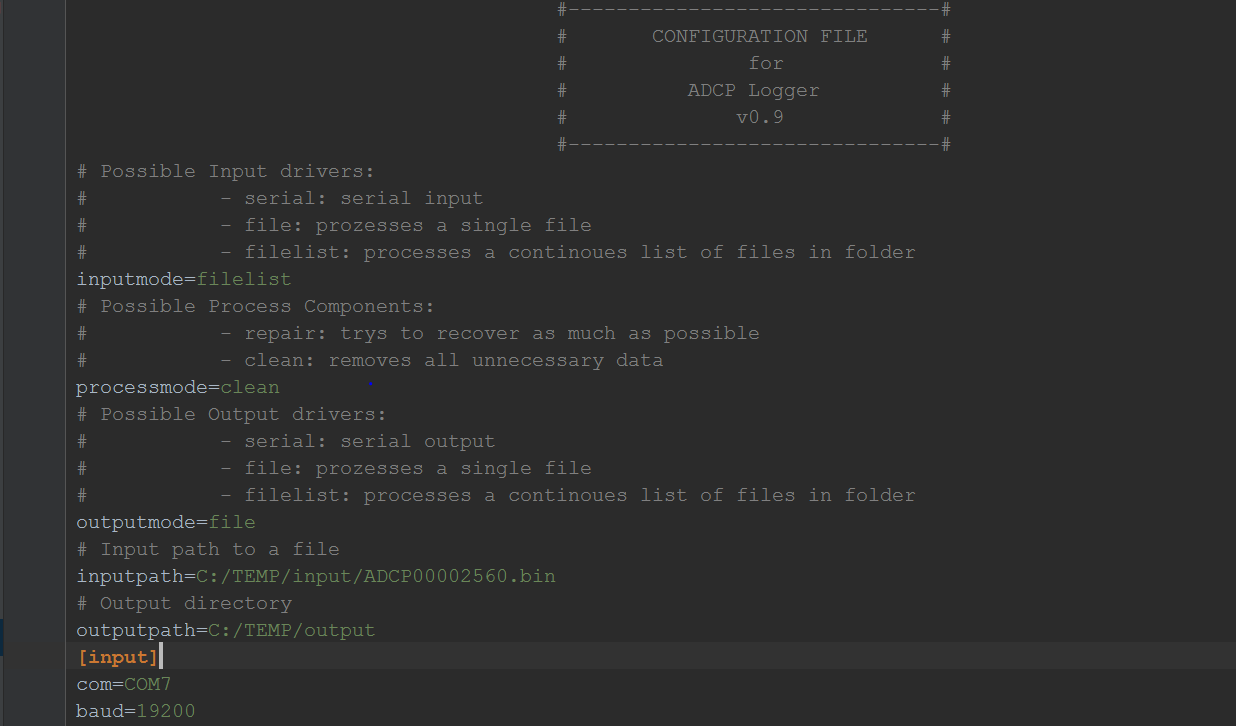
\includegraphics[width=0.7\textwidth]{config}
        \caption{A Snippet of a configuration file for the ADCP logger application}
\end{figure}

Each pipeline step is implemented as a thread. Figure 4.2 shows a dataflow model where the circles represent the threads. 
\begin{figure}[h]
\centering
      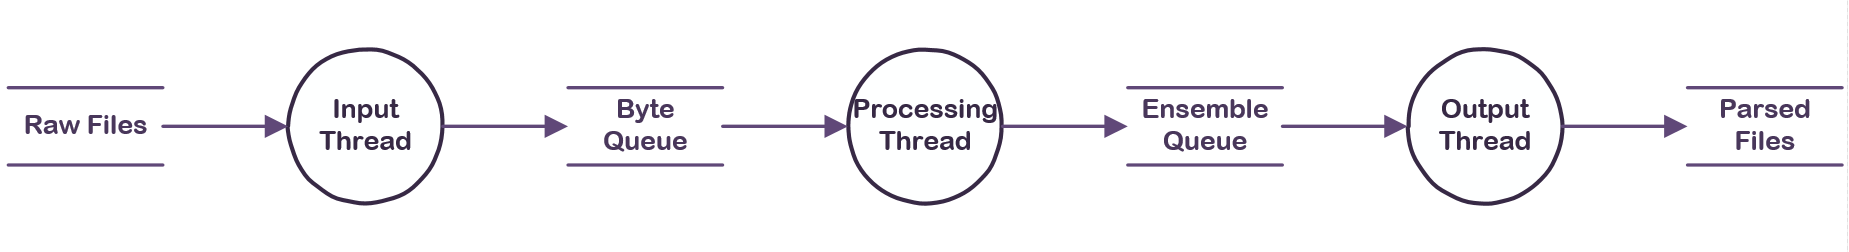
\includegraphics[width=0.95\textwidth]{dfd}
        \caption{A high-level Data-Flow-Diagram }
\end{figure}

 All threads are connected over moodycamels lockfree concurrent queues [], in the figure represented as data store objects. The queues are set up as Single-Producer-Single-Consumer (SPSC) queues and use explicit producer and consumer tokens to maximise performance. Figure 4.3 shows how the token is used to deque elements from an input queue.\\
\begin{figure}[h]	
\centering
      
\includegraphics[width=0.95\textwidth]{ct}
        \caption{Codesnippet showing the use of consumer tokens}
\end{figure}

The threads run concurrently until the end of the execution. Each thread exits if its predecessor is finished. If this is the case, the thread synchronises with its predecessor over an atomic boolean value. A speciality here is, that the memory state of the predecessor gets propagated to the thread recieving the exit signal. In the implementation the new C++11 \texttt{std::atomic\char`_thread\char`_fence} memory barriers. This step is needed so that the thread determined to exit can reliably see if it's input queue is empty. The critical function here is the \texttt{moodycamel::size\char`_approx()} function. It returns the correct size of the queue only if the memory effects of the enqueue operations in the predecessor threads have propagated. With the use of the described memory fences this state can be reliably provided. How this was implemented is shown in figure 4.4\\
\begin{figure}[h]
\centering
      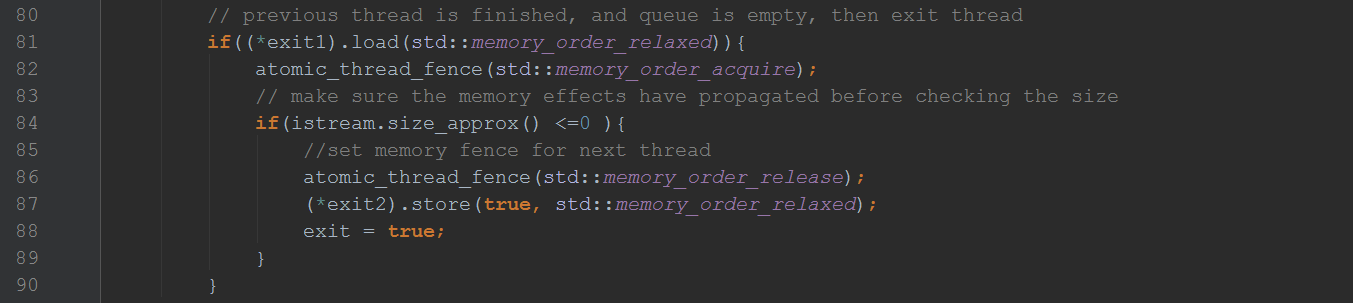
\includegraphics[width=0.95\textwidth]{memory_barrier}
        \caption{Codesnippet highlighting the memory barriers}
\end{figure}





%-------------------------------
\chapter{Testing}


 
%\input{.tex}
%\input{.tex}
\chapter{Evaluation}
This chapter will evaluate the performance and scalability of the implemented solution in terms of execution time, memory consumption, and power consumption in Section 5.1. Later on in Section 5.2 the results of the implementation are compared to the requirements from General Acoustics e.K. and finally, a comparison to similar existing ADCP solutions is presented.

\section{Performance and Scalability}
In this section, the performance of the implemented solution as well as its scalability will be tested and evaluated. First, the setup on which the tests were executed will be presented, then the assessment in terms of performance, memory consumption, and power consumption will be discussed. 
\subsection{Setup}
The measurements of the developed software were executed on three different computing stations. Two high performance devices were used to test different software configurations and acquire execution speed results while post processing old ADCP data. To test the real-time parsing of ADCP data with energy consumption in mind, a Linux driven low-power device was used.

The device with the most advanced hardware was a custom built computer with an Intel Core 6th generation i5 processor \cite{i5} over-clocked to 4.3 GHz. It had 32 GB double data rate fourth-generation (DDR4) memory \cite{ddr4} and one of the fastest solid state disk (SSD) currently available, claiming 2200 MB/s reading speed and 900 MB/s writing speed \cite{ssd}. This device was built to withstand high CPU loads, and was chosen to configure the parameters of the application and to stand as reference point for measurements with other devices.

To get performance results from a second device a Surface Book with Intel Core i7 CPU clocked at 2.6 GHz was used \cite{sb}. It had 16 GB DDR4 memory and also a fast SSD but not quite as fast as from the custom built computer (measured around 1600 MB/s read- and 600 MB/s write-speed). The results of the measurements on the Surface Book were used to compare the results from the main measuring device and, thus, gather a better impression of the overall performance of the ADCP parser application.\\
The real-time parsing requirement R1 of Section 3.1 of the software was evaluated with a BananaPro. The BananaPro has a ARM Cortex-A7 Dual-Core CPU and 1 GB DDR3 memory \cite{bpro} and runs a stripped Debian Linux derivate called Bananian Linux \cite{bananian}, it allows the configuration of the BananaPro's hardware. It has to be powered over a universal serial bus (USB). The serial port capability was enabled with a universal asynchronous receiver transmitter (UART) to USB adapter, which communicates over the RS-232 interface. To measure voltage and current flow, a USB multimeter was used \cite{mul}. Other measuring instruments to calculate a more exact energy consumption value like an oscilloscope were not available.

The different computing capabilities of the three devices allowed the evaluation of the software in terms of scalability. Scalability in this context refers to the ability of the software to adapt itself depending on the available hardware and use it accordingly.
%%%%%%%%%%%%%%%%%
\subsection{Performance}
In the evaluation of the software project, the performance of the application has an important role. Eventually the performance decides about the usability of the solution in real world scenarios and therefore, it was tested and evaluated extensively. Performance in this context relates to the execution time of the application.\\
Before any measurements were taken, the application had to be configured properly depending on the hardware and the use case. In the configuration file are a few important settings that have to be considered carefully to optimize the performance.
\begin{itemize}
\item The size of the \texttt{SequenceBuffer} (described in Section 4.2) used in the processing thread, it should at least be larger than the ADCP frame start sequence, to prevent a deadlock. Ideally, it should be larger than two times the size of the biggest ADCP frame that may be processed to prevent the processing thread from constantly auto discarding a few bytes in order to find the next start sequence.
\item The size of the Moodycamel queues used to connect the threads. If they are set wrongly the application may slow down drastically due to congestion. To avoid confusion the two queues connecting the threads were numbered: (1) is the first queue, it is a byte queue and connects the input thread to the output thread, (2) is the second queue a and contains binary messages, it connects the processing- to the output thread.
\end{itemize}

For further calculations, an average ADCP frame size of the data to be processed, was needed. The old ADCP data that was used for the performance tests had a 3992 Byte frame size for the horizontal ping, and a 992 Byte frame size for the vertical ping. The sum of both sizes was divided by two to get an average frame size of 2492 Byte. For the sake of simplicity further measurements in this report assumed an average frame size of 2500 Byte, which allowed simpler calculations.\\
Based on this average frame size, an estimate on the minimal buffer size needed was simple, it should at least be 5000 Bytes, to prevent deadlock and initial auto discarding.

The best sizes for the thread connecting queues could not be estimated easily. It could be sad that the first queue that connects the input- with the processing thread and holds the data as bytes, needs to be big enough that the processing thread can always dequeue data as needed and, thus, does not have to wait on data. Otherwise it could be assumed that the number of frames in the first queue should be equal or bigger than the number of messages in the second queue to avoid congestions.\\ 
To verify this assumptions, and get concrete numbers for the best queue sizes, a measurement was started. A bit more than one day ADCP data, exactly 150 bursts, were parsed over and over again under different queue size combinations. The execution time of each application call was written to the command line by the application and redirected into a file. The ADCP data was parsed over 1300 times, starting with very small queue sizes of 2 frames or messages in in the queues up to 400 frames or messages. \\
It had to be considered that a frame is enqueued as a number of bytes in the byte queue (1) and a message is enqueued as one object into the message queue (2). The conversion of a frame to the required number of bytes was done with the averaged frame size of 2500 Byte from above and, thus, if the first queue should contain 5 frames, the size should be set to 5 $\times$ 2500 = 12500 Byte.

\begin{figure}[hb]
\centering
      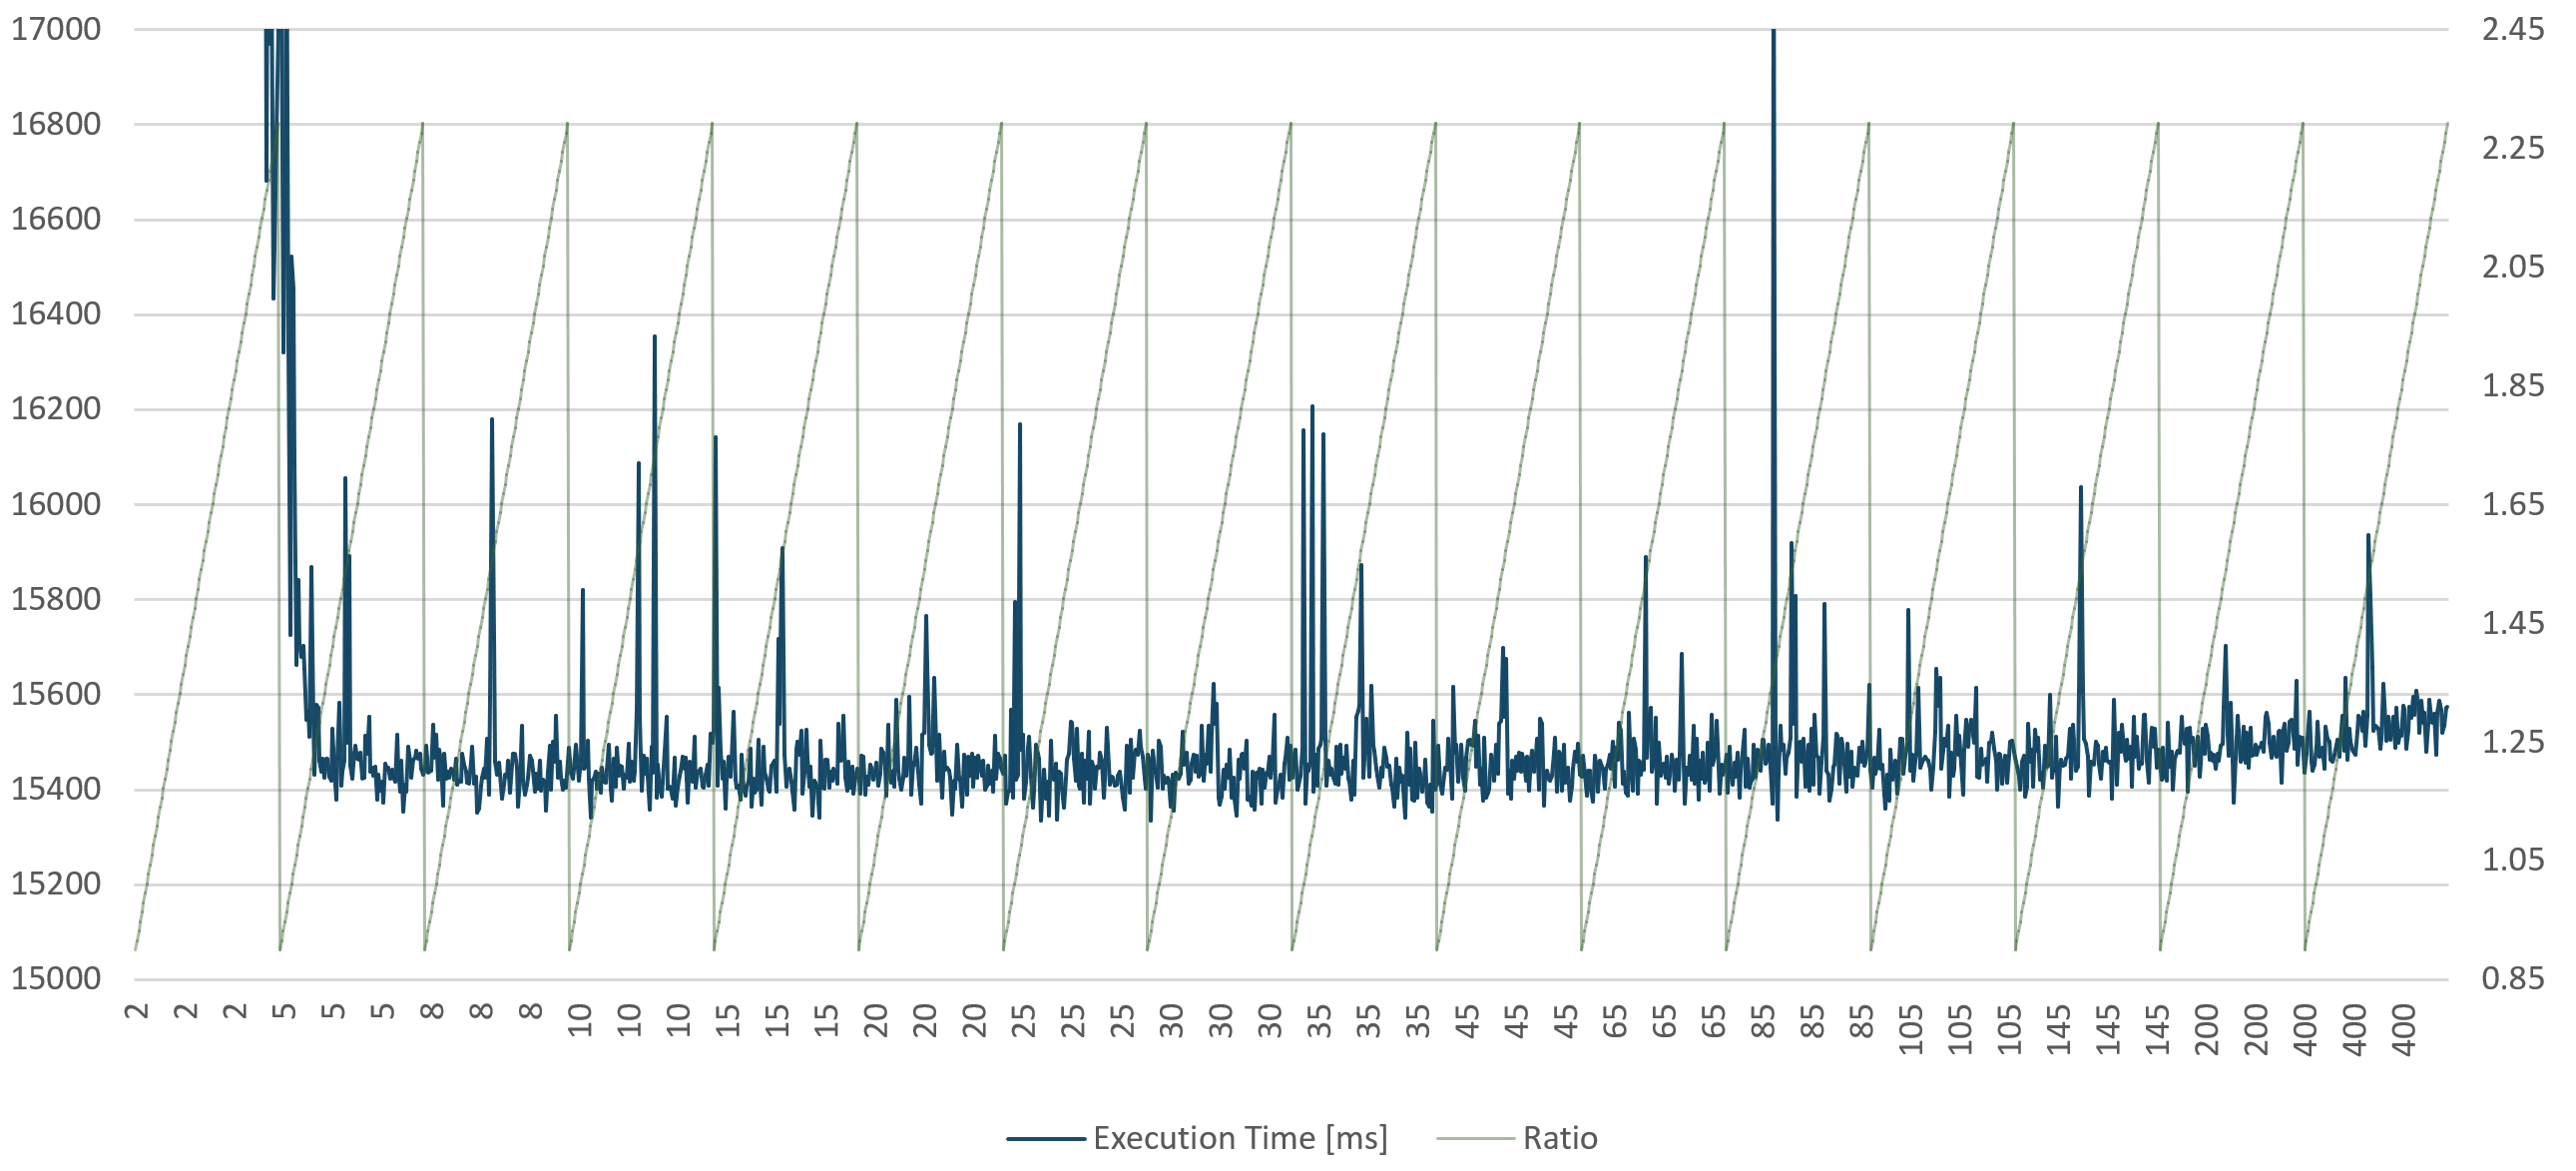
\includegraphics[width=1\textwidth]{conf_main}
        \caption{Measurement of 150 ADCP bursts under various queue configurations on a desktop computer}
\end{figure}

In the measurement, not only the number of frames in the queues were varied, but also the ratio between these queues was varied. The size of the first queue was varied between 90\% and 230\% of size from the second queue. Figure 5.1 presents the results, the light-blue zigzag line displays the ratio of the first queue (1) to the second queue (2), the darker line presents the measured time in milliseconds. The x-axis shows the number of frames in the message queue (2). It can be seen that, if the queue sizes were under five frames the measured times were visibly slower, but with values larger than five frames in the queues, the execution speed varied only around 5 percent. The outliers appeared to be random and may come from additional workload through background tasks of Windows. It can be concluded that the queue sizes should not be to low to avoid the congestion, but the selected ratio does not play a big role performance wise. Surprisingly the use of more memory due to bigger queues does not improve the performance after the minimal required queue size is reached, thus it can also be concluded that the performance limiting factor was not the memory consumption of the software.

To select a default value of the queue sizes for the configuration file, the ratio between the queues of the 50 fastest execution times were averaged. Table 5.1 shows the 20 fastest measures with its respective queue sizes. The average value over the 50 measure points was added at the end. 

\begin{table}[!]
\centering
	\begin{tabular}{l|c|c|c}
	  \hline
	  	&\textbf{Execution Time} & \textbf{Ratio (1)} & \textbf{Framenumber in(2)}\\\hline 
	  	& 15335.1 ms & 1.268 & 25\\
		& 15335.1 ms & 0.932 & 30\\
		& 15336.2 ms & 1.396 & 85\\
		& 15337.9 ms & 1.428 & 25\\
		& 15341 ms  & 1.924 & 15\\
		& 15341.4  ms & 2.004 & 35\\
		& 15341.7  ms & 1.108 & 10\\
		& 15345.9  ms & 1.86 & 15\\
		& 15346 ms & 1.764 & 30\\
		& 15346.5  ms& 1.348 & 25\\
		& 15348.5  ms& 1.812 & 20\\
		& 15352.8  ms& 1.412 & 8\\
		& 15353 ms  & 2.1	 & 5\\
		& 15353 ms  & 2.26 & 35\\
		& 15355.3 ms & 2.084 & 8\\
		& 15355.3 ms & 1.156 & 30\\
		& 15357.1 ms  ms& 1.94 & 30\\
		& 15357.7 ms & 1.684 & 10\\
		& 15358.2 ms & 2.084 & 25\\
		& 15358.3 ms & 1.684 & 15\\
		& \dots & \dots & \dots\\\hline
	  	\textbf{Average} & 15359.5 ms& 1.61 & 34.5\\ 
	  \hline
	\end{tabular}
	\caption{The 20 fastest execution times with the respective ratio and queue size}
\end{table}

To verify the measured behavior, the same test was executed on the Surface Book, Figure 5.2 presents the results in a similar graphic than already explained for Figure 5.1, it can be seen that the execution time is slower around 7 seconds, and varies much more than in Figure 5.1. The time varies between 22.5 seconds and 25.5 seconds, but a clear bias can be seen towards 22.75 second. This behavior may result from CPU throttling due to thermal issues and, thus, it can be concluded that a mobile CPU as used in the Surface Book is not the best choice for heavy data processing. Nonetheless the results confirm that the application does not depend on the amount of memory used after exceeding the minimal required queue size. They also confirm that the ratio between the queues has no big impact on the execution time as already seen in Figure 5.1. 
\vspace{1em}

\begin{figure}[h]
\centering
      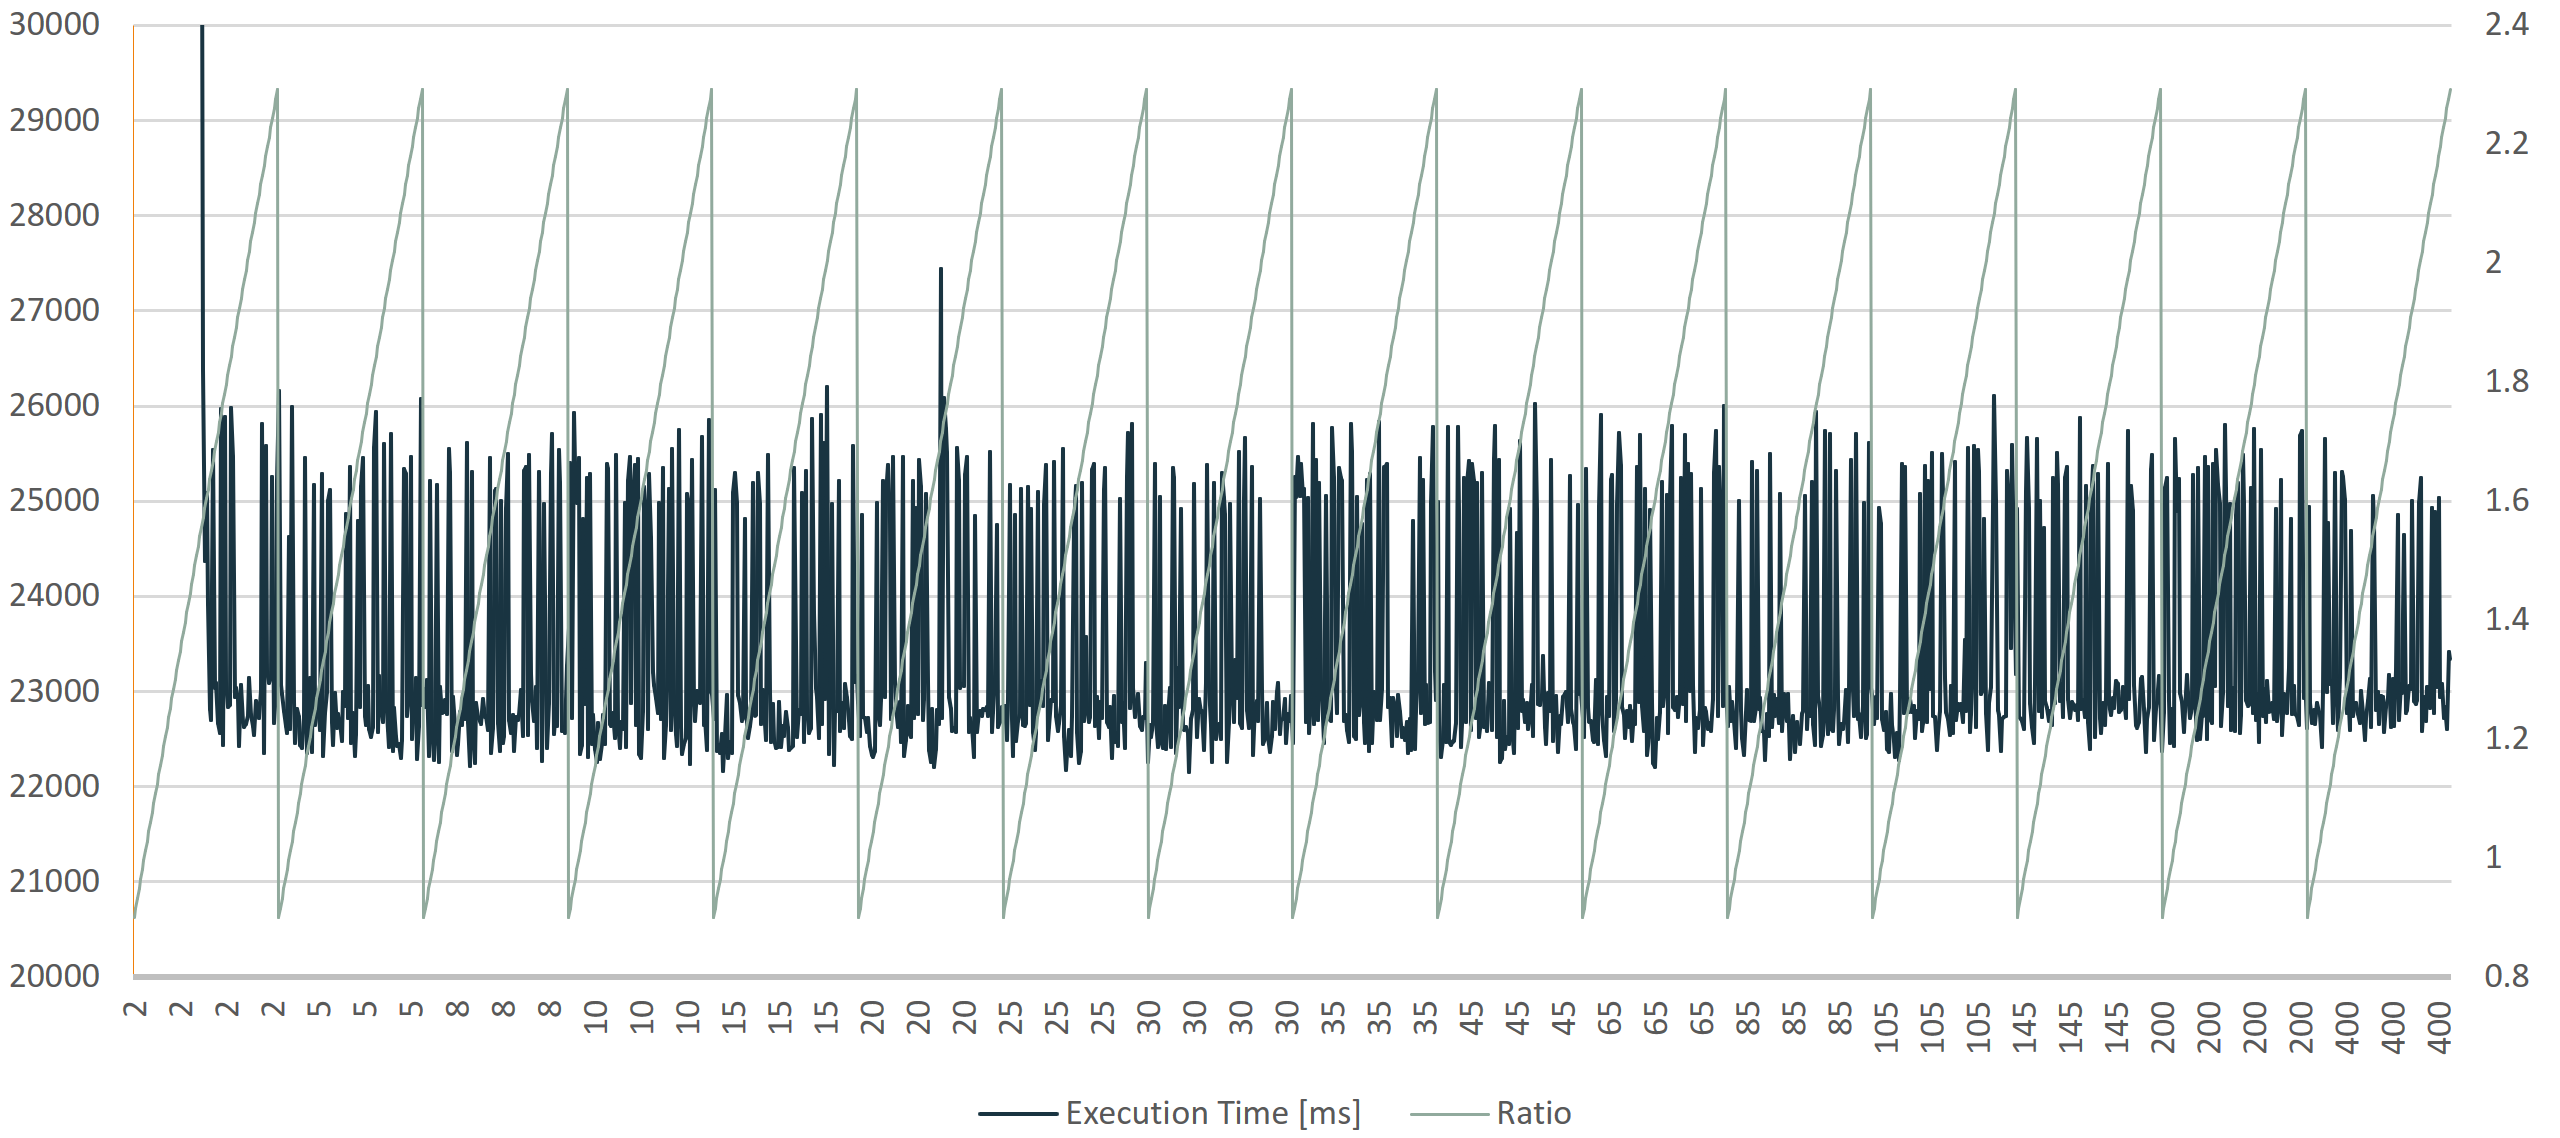
\includegraphics[width=1\textwidth]{conf_sb}
        \caption{Measurement of 150 ADCP bursts under various queue configurations on a Surface Book}
\end{figure}

To reassess the new found memory independence, a new measurement was executed. This time the fixed size ratio of 1.6 as calculated in Table 5.1, was used between the queues. Once again sizes between two and 400 frames in the message queue were measured in 90 steps five times. The averaged results are presented in Figure 5.3, it can be seen that the execution (orange line) time even gets slightly poorer if the queue sizes (on the x-axis) grow over 80 frames, which may result from slower performance of the Moodycamel queues if they are allocated to big, but remain empty most of the time.
\vspace{1em}

\begin{figure}[h]
\centering
      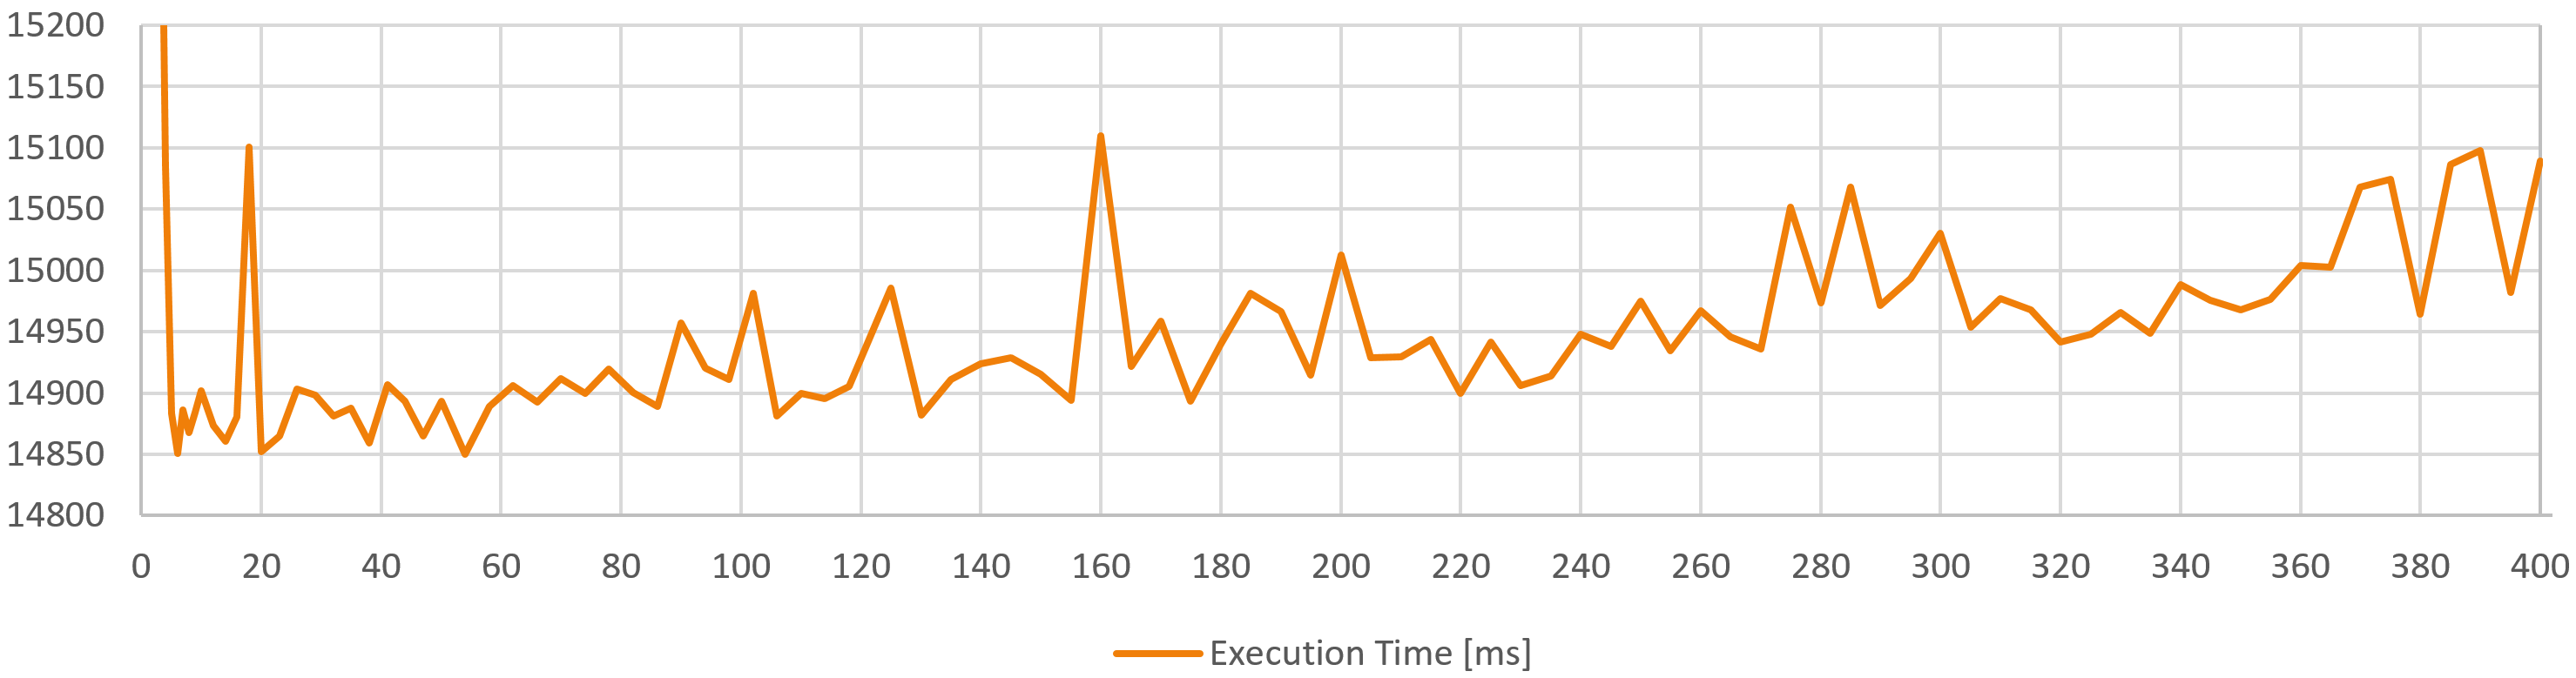
\includegraphics[width=1\textwidth]{perf_mem_1}
        \caption{Impact of extensive memory usage on the execution time}
\end{figure}

\pagebreak
After seeing that the memory consumption did not have a big impact on performance some general tests were done where different amounts of old data was parsed at a fixed configuration of 30 frames in the message queue (2) and a ratio of 1.6 for the byte queue (1). Table 5.2 presents the resulting figures. 

\begin{table}[!h]
\centering
	\begin{tabular}{|l|c|c|}
	  \hline
	  	\textbf{Device} & \textbf{Desktop Computer} & \textbf{Surface Book}\\ \hline
	  	\textbf{10 Minutes (5 MB)} & 152 ms & 238 ms\\
	  	\textbf{1 Day (700 MB)} & 14.9 s & 20.95 s\\
	  	\textbf{1 Week (4.9 GB)} & 104.3 s & s\\
	  \hline
	\end{tabular}
	\centering
	\caption{Execution time at a fixed configuration and various amount\\ of data on the desktop computer and the Surface Book}
\end{table}

With this performance three years of old ADCP data could be parsed in under 5 hours, resulting in around 105 ms per 10-minutes burst. It can be concluded that this performance satisfies all needs in terms of post processing.

To complete the post processing requirement measurements, the BananaPro was also used to post-process some old ADCP data. The results shown in Table 5.3 show really slow execution times of around XXX seconds per ADCP frame. The results are understandable, as the processor has not the power to do extensive data processing and was not built for it.

\begin{table}[!h]
\centering
	\begin{tabular}{|l|c|}
	  \hline
	  	\textbf{Device} & \textbf{BananaPro}\\ \hline
	  	\textbf{10 Minutes (5 MB)} & 8.1 s \\
	  	\textbf{1 Hour (30 MB)} & 47.8 s \\
	  \hline
	\end{tabular}
	\begin{center}
			\caption{Execution time at a fixed configuration and various amount\\ of data on the BananaPro}
	\end{center}
\end{table}

The memory consumption can be ruled out as performance critical bottleneck if a queue size larger than five frames is used. The real bottleneck in the current implementation is the processing thread, on the main computer, the core running the processing thread was always busy at 100\% whereas the overall CPU load never exceeded 65\%. Currently the processing thread does all CPU intensive work, it converts the ADCP frames to ADCP ensembles containing integers and floats, then cleans the data, and converts the ensemble back to a frame and later completely to bytes. The idea of this implementation was the preparation for further processing steps. For example, if a second processing step would be implemented for wave analysis, the first processing thread would only convert the data to ADCP ensembles, and pass them to the second thread, where they would used further. In the last part of Chapter 6 a solution to improve the current design is described.

\subsubsection{Real-Time Parsing} 
The real-time processing, was tested first under Windows. A pair of virtual COM ports was used to test high data throughput with a Baud rate of 468000 Bd. This Baud rate is also used for the real ADCP communication over an RS-485 interface. The application run flawlessly consuming 5 MB memory and one percent CPU usage, even with five times of the data that would be generated by an ADCP.\\
The tests with the BananaPro had to be done over RS-232 interfaces as no appropriate RS-485 hardware was available. The RS-232 adapters used allowed a maximum Baud rate of 115200 Bd, this was just enough to receive two times the data that would normally be generated by an ADCP.\\
On the BananaPro the application used again around 5 MB memory, and burdened the CPU with a maximum of 3 percent CPU load. The reached performance is really good, as the data to be processed from a real ADCP would be lower and, thus, the CPU load would be as well lower.
\subsection{Memory Consumption}
The memory handling of the software is straight forward. Most objects are allocated on the stack and eventual memory leaks of the heap were carefully eliminated, as the software may have to run infinitely and must not grow. After all components are instantiated, the allocated memory oscillates only very little, even if the application runs idle. The reason is, that most objects of the software are rather allocated once and overwritten, than destroyed and reallocated. Another reason is, all data structures are preallocated and prohibited to grow. This circumstance means that the maximal memory consummation can be estimated before running the application.\\
\begin{figure}[h]
\centering
      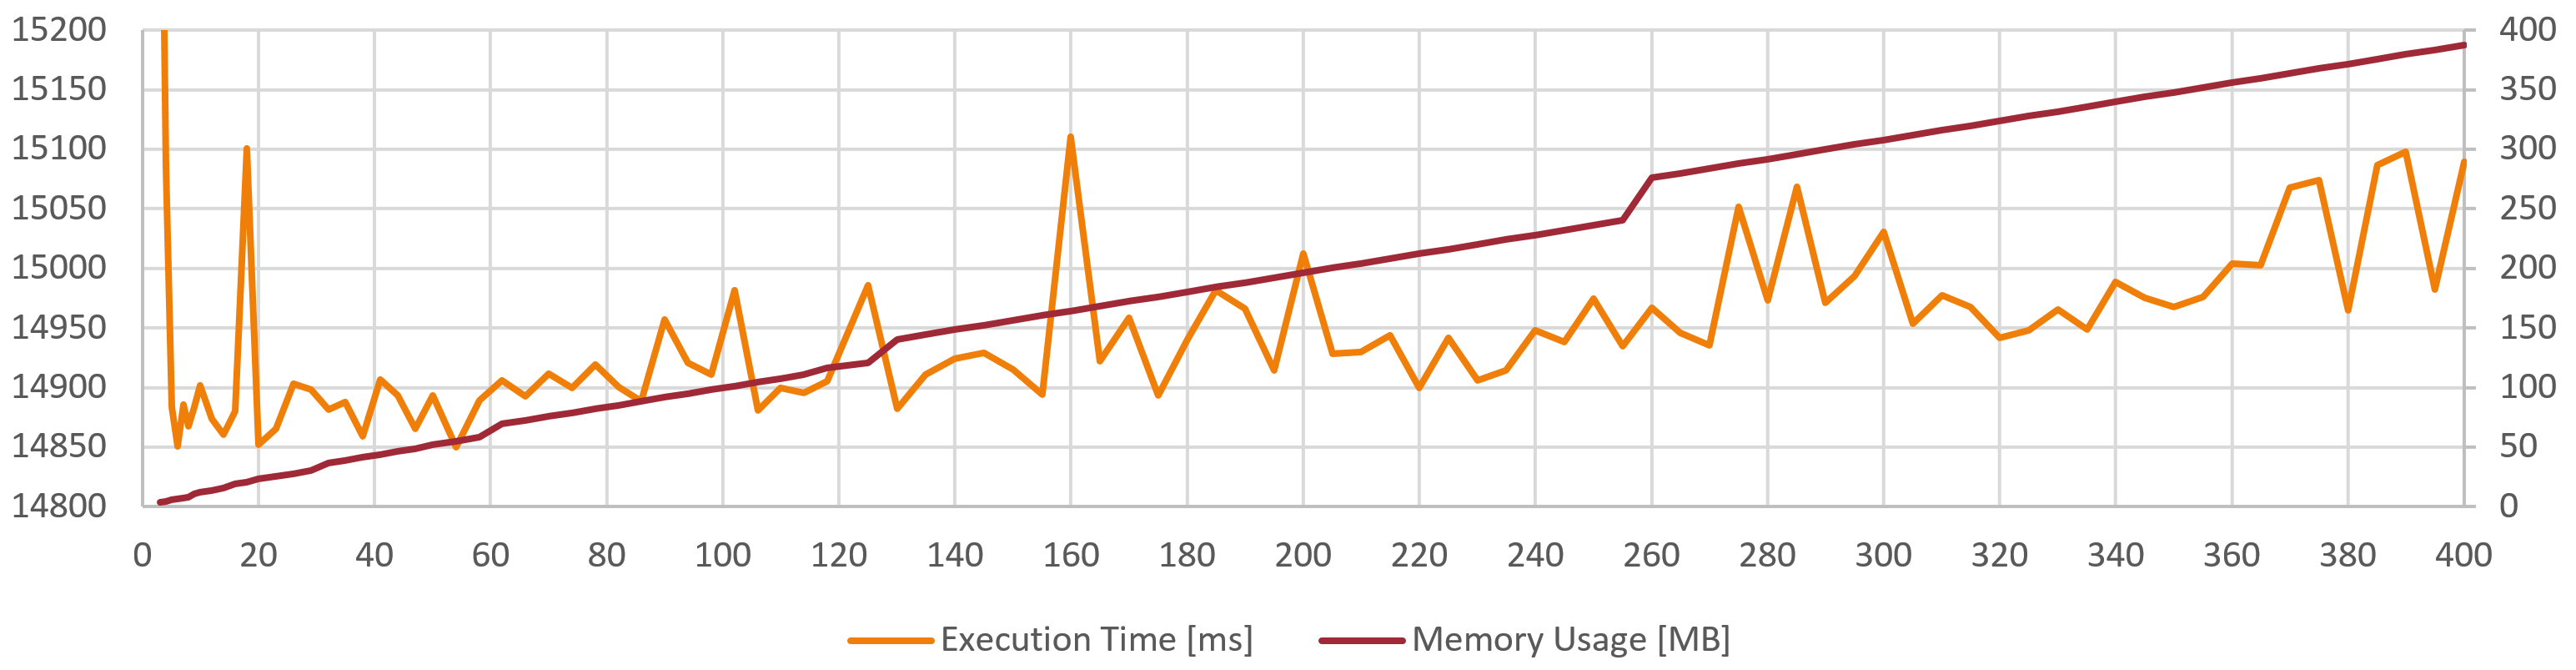
\includegraphics[width=1\textwidth]{perf_mem_2}
        \caption{Memory Consumption and execution time for various queue sizes}
\end{figure}

Figure 5.4 shows the memory consumption of the test run shown in Figure 5.3 from the previous Section 5.1.2, one can see that the memory grows equally with the preset sizes of the queues. With the average ADCP frame size of 2500 Byte calculated in Section 5.2.1 and the  it is possible to calculate the number of estimated ensembles in the system. To simplify this calculation it was assumed that only the ensembles in the byte queue from the input thread to the processing thread, as well as the message queue from the processing thread contain ensembles. The ensembles currently floating in the three threads were ignored.\\
The estimated ensemble number was compared against the actual memory consumption. It can be seen that an ensemble in the application requires around 0.45 MB memory, in Figure 5.3 the red line represents the used memory per ADCP ensemble. The value is high, 128 times of the estimated ensemble size. The reasons are, (1) the previously ignored `floating' ensembles in the threads come into play. If the queues are full, the input thread holds a buffer containing 30 percent of the data in the byte queue and the processing thread holds also a multiple of the currently processed ensemble e.g. in form of MATLAB matrices. Also (2) the Moodycamel queues preallocate their memory in a way that all threads are always able to execute their desired nonblocking operation. This requires to maintain more memory than actually needed. 

\subsection{Power Consummation}
In Section 5.1.2 the performance of the software on the BananaPro was assessed in terms of speed, there, it was shown that the BananaPro is not made for batch-processing of old ADCP data, but that it is fast enough by far to process real-time data. It was also shown that the configuration for the BananaPro in real-time parsing mode works well with as few as 4-5 MB memory, and almost never exceeds CPU usage of more than 3 percent.\\ 
The missing information about the power consummation of the BananaPro was measured with the USB multimeter described in Section 5.1.1. First the voltage and current was measured when the BananaPro was idle and then while executing the application. During the measurements the power adapter was changed because the old one could only deliver 750mA at 4.9 V which lead to variations of 60 mA. With the new power adapter which could deliver up th 2.4 A, no more ups and downs could be measured. Table 5.x presents the results of the measurements with the new power adapter, with a stable voltage, and a difference of 10 mA for the current. The multimeter only had a 10 mA resolution and therefore the measurement is not very exact, but it shows at least that the power consumption does not exceed 10 mA which is a maximum 3.5 percent of the overall power consumption.

\begin{table}[h]
	\centering
	\begin{tabular}{l@{\quad}c@{\quad}c@{\quad}c@{\quad}c} \hline \rule{0pt}{8pt}
	  %Component & Total RAM & Payload size & IPFIX package size \rule{0pt}{12pt} \\ \hline \rule{-2pt}{12pt}
	  & Idle & Real-Time Parsing \rule{0pt}{8pt} \\\hline \rule{-2pt}{8pt}
	  volatge [V] & 5.24 V & 5.24 V\\
	  current [mA] & 280 mA& 290 mA\\ 
	  \hline
	\end{tabular}
	\caption{Comparison of power consummation on the BananaPro, between idle and parsing real time ADCP data.}
	\label{tab:energy}
\end{table}

\section{Software Project Results}
The goal of this software project was the design and the implementation of a modular ADCP parser as stated in Section 1.1. This software project was done in cooperation with General Acoustics e.K. and had to follow their requirements described in Section 3.1. The implemented solution was compared to these requirements and the results were presented in Table 5.1.

\begin{table}[ht]
\centering
	\begin{tabular}{|l|l|}
	  \hline
	  	\textbf{Requirement R1} 
	  	& The software should be able to parse real time ADCP\\ 
	  	& data on a low-power data logger, clean it by removing unused\\
	  	& information and, thus, enable the possibility of logging longer\\
	  	& time periods due to the reduced size.\\ \hline
	  	\textbf{Result} 
	  	& Fully completed and tested with virtual serial ports and\\ 
	  	& high Baud rates (460800 Bd) and data throughput on a high \\ 
	  	& performance Windows system, as well on a low-power ARM7 \\ 
	  	& BananaPro with a real RS232 serial port and hardware \\ 
	  	& restricted 115200Bd. The test setup is further described \\
	  	& in Section 5.1.2.\\
	  \hline
	  \hline
	  	\textbf{Requirement R2} 
	  	& The possibility of processing old raw data files with focus\\
	  	& on speed rater than efficiency.\\ \hline
	  	\textbf{Result} 
	  	& Fully completed, and tested with various old data files. \\
	  	& Measurements on the performance can be found in section 5.1.2.\\
	  \hline
	  \hline
	  	\textbf{Requirement R3} 
	  	& The application should scale according to the available\\
	  	& hardware.\\ \hline
	  	\textbf{Result} & Completed through a threaded approach.\\
	  \hline
	  \hline
	  	\textbf{Requirement R4} 
	  	& The software should be portable. \\ \hline
	  	\textbf{Result} 
	  	& Completed, the application was written in C++11 with the\\
	  	& help of Boost libraries, and is completely platform\\
	  	& independent.\\
	  \hline
	  \hline
	  	\textbf{Requirement R5} 
	  	& Save electricity to go easy on the battery if operated by one.\\ \hline
	  	\textbf{Result} 
	  	& Completed, the use of the low-level programming language\\
	  	& C++ resulted in a high performance application that uses as\\
	  	& little as possible processing time in real time parsing. \\
	  \hline
	  \hline
	  	\textbf{Requirement R6} 
	  	& The application should allow additional processing steps apart\\
	  	& from the parsing.\\ \hline
	  	\textbf{Result} 
	  	& Completed, the threaded component based approach from\\
	  	& Section 3.2 fulfills this requirement.\\
	  \hline
	  \hline
	  	\textbf{Requirement R7} 
	  	& The architecture should allow other sensor types without\\
	  	& having to change sensor unrelated code.\\ \hline
	  	\textbf{Result} 
	  	& Completed, it would be possible to switch all ADCP related\\
	  	& code with components from another sensor, and the application\\
	  	& would work in the same manner.\\
	  \hline
	  \hline
	  	\textbf{Requirement R8} 
	  	& The software should be implemented in a well structured\\
	  	& component based approach.\\ \hline
	  	\textbf{Result} & Completed \\
	  \hline
	  \hline
	  	\textbf{Requirement R9} & The components should be decoupled as much as possible.\\ \hline
	  	\textbf{Result} & Completed \\
	  \hline
	  \hline
	  	\textbf{Requirement R10} 
	  	& Components with no dependency to the ADCP context should\\
	  	& be implemented as completely independent components\\ \hline
	  	\textbf{Result} 
	  	& Completed, MATLAB component \texttt{MatlabUtils}, sequence\\
	  	& buffer \texttt{SequenceBuffer}, and binary input and output\\
	  	& \texttt{BinaryIO} are implemented completely independent.\\
	  \hline
	\end{tabular}
	\caption{asdsad}
\end{table}

In addition to the implementation specific requirements, the code should also be properly documented to satisfy the expectations of General Acoustics e.K., particularly Jan Schirrmacher as he has to work with the solution in the future. The documentation was completed and signed off by Jan Schirrmacher.\\
The Correctness of the software was tested through intensive parsing of real ADCP data in various modes and compare the results with results generated from a already tested parsing software developed by General Acoustics e.K. on Windows. To test the behavior on predefined error cases, a simple testing software was constructed that generates bursts of ADCP data with or without errors, and outputs them to a serial port. The source code of this testing application was included in Appendix B, it uses a lot of components developed in this software project. With this application the behavior on missing byte errors can be understood. Such errors happen often when the serial connection from the ADCP to the logger is bad, and was in recent projects the biggest point of failure for corrupted ADCP data.\\
The application reacted as expected, in the cleaning mode, it only considered frames that were completely intact and ignored frames with failures. If the application was run in repair mode, it tried to correct errors and returned frames that could be repaired. For the repair functionality it was essential that the number of missing bytes did not exceed two bytes per ensemble matrix, otherwise the possibility of wrong values that are semantically correct, rises, and the quality of the data can not be guaranteed.\\

\subsection{Comparison to Similar Solutions}
The software developed in this software project can be seen as very exotic. Outside from the field where General Acoustics e.K. is active, ADCP's are rarely known, and according software not existent. ADCP distributors either include the parsing and wave processing in the hardware, or distribute proprietary software with the ADCP. The producer of the reference ADCP used in this project gives access to the source code of its ADCP configuration and analyzing software written in for Windows in C\# \cite{rowe_git}. This software can be used to look at, and store ADCP data, but has huge performance issues and can hardly be compared to the software developed in this software project. It was also meant to be used for the configuration of the ADCP and not for the data processing.\\
Other possibilities where the result of the software project could be compared against, were applications produced by General Acoustics e.K.. The problem here was, that the ADCP related algorithms were always included in other bigger graphical applications and, thus, not suitable for direct comparison. One software can parse ADCP data and returns a human readable MATLAB ready text file with the parsed matrix data. Because the application writes a file, and at the same time outputs information about the data on the display, it was massively slower than a command line application like the software implemented in this software project.

The software as it was implemented stands alone and can not really be compared to anything existing yet. 

Currently available software either from General Acoustics e.K. nor from Rowe Tech. Inc. cannot reach this performance by far. A direct comparison to these tools was not done, the software from Rowe Tech. Inc. was written in C\# and performs badly but was only thought to configure the ADCP and look at some data to verify that the ADCP was configured properly. The parsing software from General Acoustics e.K. was included in different applications, e.g. for graphical representation of the data or directly connected to a database.   




\chapter{Summary and Conclusions}
In the course of this software project, a modular application to parse ADCP data was designed and developed for General Acoustics e.K residing in Kiel, Germany. The design was guided by requirements posed by General Acoustics e.K.. The result of the design was a component based ADCP parser built upon a threaded pipeline architecture to enhance scalability. The design is flexible and allows the addition of new functionality either as an additional components that can be executed by one of the existing threads, or as new step in the pipeline in form of an additional thread. The application features the possibility of real-time data parsing on incoming data on a serial port as well as the ability to parse old ADCP data files. Additionally it is also able to repair faulty ADCP data.\\
The implementation was done in modern C++11, new optimizing features like move semantics and shared pointers were used intensively. Each component was developed as independent as possible to decouple the whole system and raise the reuse ability. The Boost C++ libraries were used to simplify the development and allow complete portability of the code.\\
The result was a application with scalable performance depending on its configuration and the used hardware. It fulfills the requirements and surpasses them by adding a repair option to fix defective ADCP data. The application built in this project can be used in a productive environment and builds a basic framework to support upcoming projects with similar requirements.\\

To conclude this software project 

The result of this soft
% The performance requirements were not  strictly predefined. Implicitly they were given through the functionality requirements. The real-time operation, as well as post-processing of a big amount of old data should be possible in reasonable time. These requirements are satisfied by far. On a actual desktop computer with a fast SSD the application parses 180 bursts in around 30 seconds which results in around 166 ms per burst. This performance is really good!. The memory used never exceeds 28 megabytes. On the low-power data-logger the performance is slower, the CPU cannot keep up. For real-time operation the performance is by far fast enough, in 40 seconds the logger is capable to process five bursts, in real-time one burst would arrive every 10 minutes. The performance could probably be optimized in dropping the well-structured object oriented approach and working more directly with memory, bit it would be a high price to pay. One would lose the flexibility of easily adding new functionality, and the whole component based approach.
% In recapitulation of the chosen threaded architecture needs to be said that multithreaded development can be really painful. Debugging this software sometimes has cost countless hours to find segmentation faults, memory leaks or uncatched exceptions. The available toolset to debug these kind of application was small. The tools were either for Microsoft's MSVC compiler or only available on Linux. For upcoming projects it would be better to develop on either one of the platforms mentioned. At least a good heap profiler should be available.
% That said, the application with its structured and decoupled code-base in conjunction with the background information delivered in this report results in a complete package. The application is ready for productive operation. The code is ready to be used in upcoming projects, be it only through adding new functionality or completely redesigning the frame around the components. And at last the report and the documented source code delivers enough background information and overview over the application for other developers to understand the problem and start working on it for further projects.  

\begin{thebibliography}{99}
\addcontentsline{toc}{chapter}{Bibliography}

\bibitem{adcp_def}Adcp user guide, \url{http://rowetechinc.co/adcp/RTI%20ADCP%20DVL%20USER%20GUIDE%20Rev%20AB.pdf}, last visit Jun 05, 2016
\bibitem{rowe}Rowe Technologies Inc., \url{http://rowetechinc.com/}, last visit Jun 05, 2016
\bibitem{boostliz} Boost Software License, \url{http://www.boost.org/users/license.html}, last visit Jun 05, 2016
\bibitem{boost_asio} Boost Asio, \url{http://www.boost.org/doc/libs/1\_61\_0/doc/html/boost\_asio.html}, last visit Jun 05, 2016
\bibitem{boost_files} Boost Filesystem, \url{http://www.boost.org/doc/libs/1\_61\_0/libs/filesystem/doc/index.htm}, last visit Jun 05, 2016
\bibitem{boost_po} Boost Program Options, \url{http://www.boost.org/doc/libs/1\_61\_0/doc/html/program\_options.html}, last visit Jun 05, 2016
\bibitem{boost_test} Boost Test, \url{http://www.boost.org/doc/libs/1\_61\_0/libs/test/doc/html/boost\_test/intro.html}, last visit Jun 05, 2016
\bibitem{boost_thread} Boost Thread, \url{http://www.boost.org/doc/libs/1\_61\_0/doc/html/thread.html}, last visit Jun 05, 2016
\bibitem{moody} Moodycamel Concurrent Queue, \url{https://github.com/cameron314/concurrentqueue}, last visit Jun 05, 2016
\bibitem{benchmark} Moodycamel Concurrent Queue Benchmark, \url{http://moodycamel.com/blog/2014/a-fast-general-purpose-lock-free-queue-for-c++#benchmarks}, last visit Jun 05, 2016
\bibitem{serport}Serial Port Wrapper, \url{https://github.com/fedetft/serial-port}, last visit Jun 05, 2016
\bibitem{clion}Jetbrain Clion, \url{https://www.jetbrains.com/clion/}, last visit Jun 05, 2016
\bibitem{intellij} Jetbrain Intellij, \url{https://www.jetbrains.com/idea/}, last visit Jun 05, 2016
\bibitem{mingw}Nuwen's MinGW, \url{https://nuwen.net/mingw.html}, last visit Jun 05, 2016
\bibitem{cpp_std}C++ Standard, \url{https://isocpp.org/std/the-standard}, last visit Jun 05, 2016
\bibitem{gtest}Google Test, \url{https://github.com/google/googletest}, last visit Jun 05, 2016

\bibitem{getop}getopt, \url{http://www.gnu.org/savannah-checkouts/gnu/libc/manual/html_node/Getopt.html}, last visit Jun 05, 2016
\bibitem{tclap}TCLAP, \url{http://tclap.sourceforge.net/}, last visit Jun 05, 2016
\bibitem{boost_lockfree} Performance of lockfree Queues, \url{http://joshitech.blogspot.ch/2015/02/queue-benchmark.html}, last visit Jun 05, 2016
\bibitem{matlab} Matlab v.4 Documentation, \url{http://www.eiscat.com/groups/Documentation/UserGuides/matlab4.pdf},, last visit Jun 05, 2016
\bibitem{stackof} Type independent vector, \url{http://stackoverflow.com/questions/36020246/type-independent-vector-class-member}, last visit Jun 05, 2016

\end{thebibliography}



\chapter*{Abbreviations}
\addcontentsline{toc}{chapter}{Abbreviations}
\markboth{ABBREVIATONS}{}


\abr{AAA}{Authentication, Authorization, and Accounting}

\chapter*{Glossary}
\addcontentsline{toc}{chapter}{Glossary}
\markboth{GLOSSARY}{}


\begin{description}
  \item[bin] Bins are the discreet values where the ADCP measures the flow. In this project a bin has the hight of 0.5 m.
  \item[beam] An ADCP has a finite number of beams. Beams emit the waves used to measure the flow currents and directions. At least 3 beams have to be available to be able to measure the direction of the flow.
  \item[ADCP ensemble] An ADCP ensemble contains all data of one measuring ping. The data is stored in a series of MATLAB matrices.
  \item[ADCP frame] An ADCP frame is essentially an ensemble with a header at the beginning and a CRC checksum at the end. The ADCP sends out frames. The frame header and the checksum allow error detection.
  \item[ADCP burst] A collection of a number ADCP frames measured continuously. In this project a burst contains 2048 frames collected over around 6-7 minutes.

\end{description}


\addcontentsline{toc}{chapter}{List of Figures}
\listoffigures
\addcontentsline{toc}{chapter}{List of Tables}
\listoftables

\appendix

\chapter{Documentation of ADCP Matrices }
The documentation of all ADCP matrices was captured as screen shots from the official ADCP user guide from Rowe Tech. Inc. \cite{adcp_def} .

\begin{figure}[ht]
\centering
      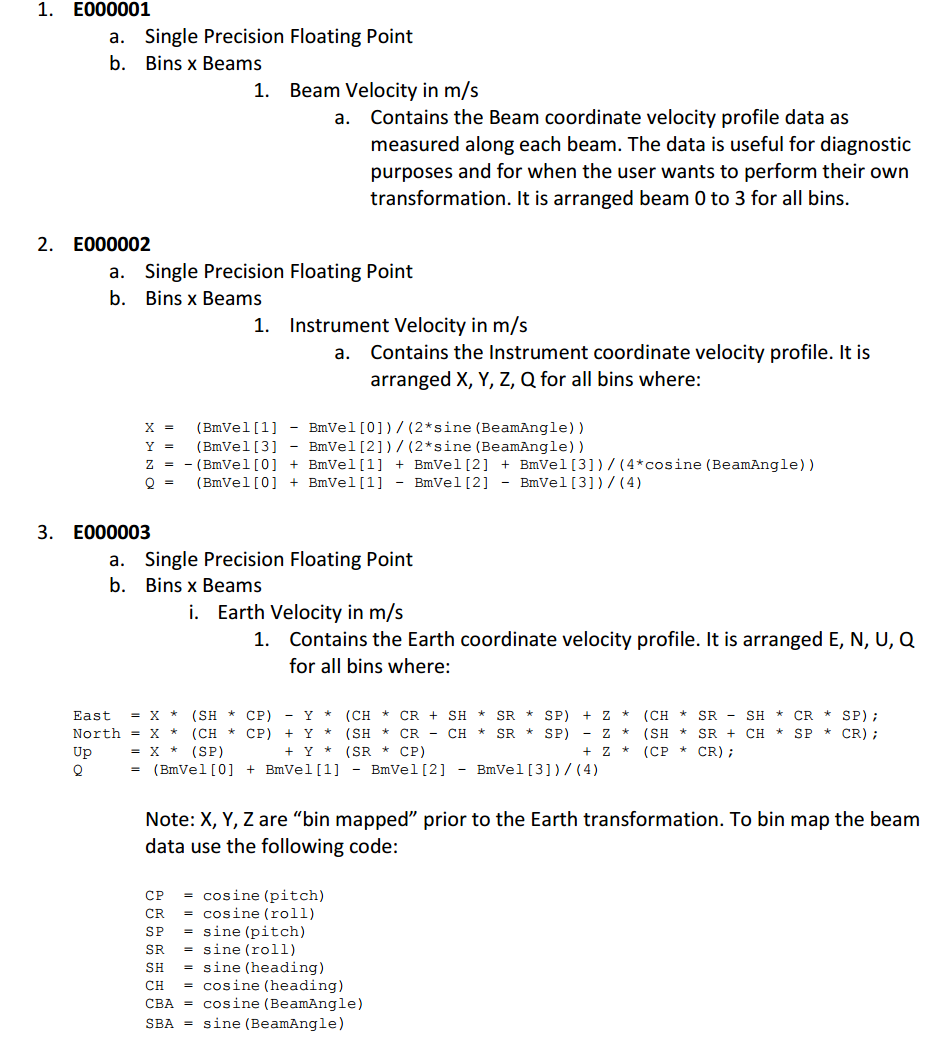
\includegraphics[width=1\textwidth]{ens1}
\end{figure}
\begin{figure}[ht]
\centering
      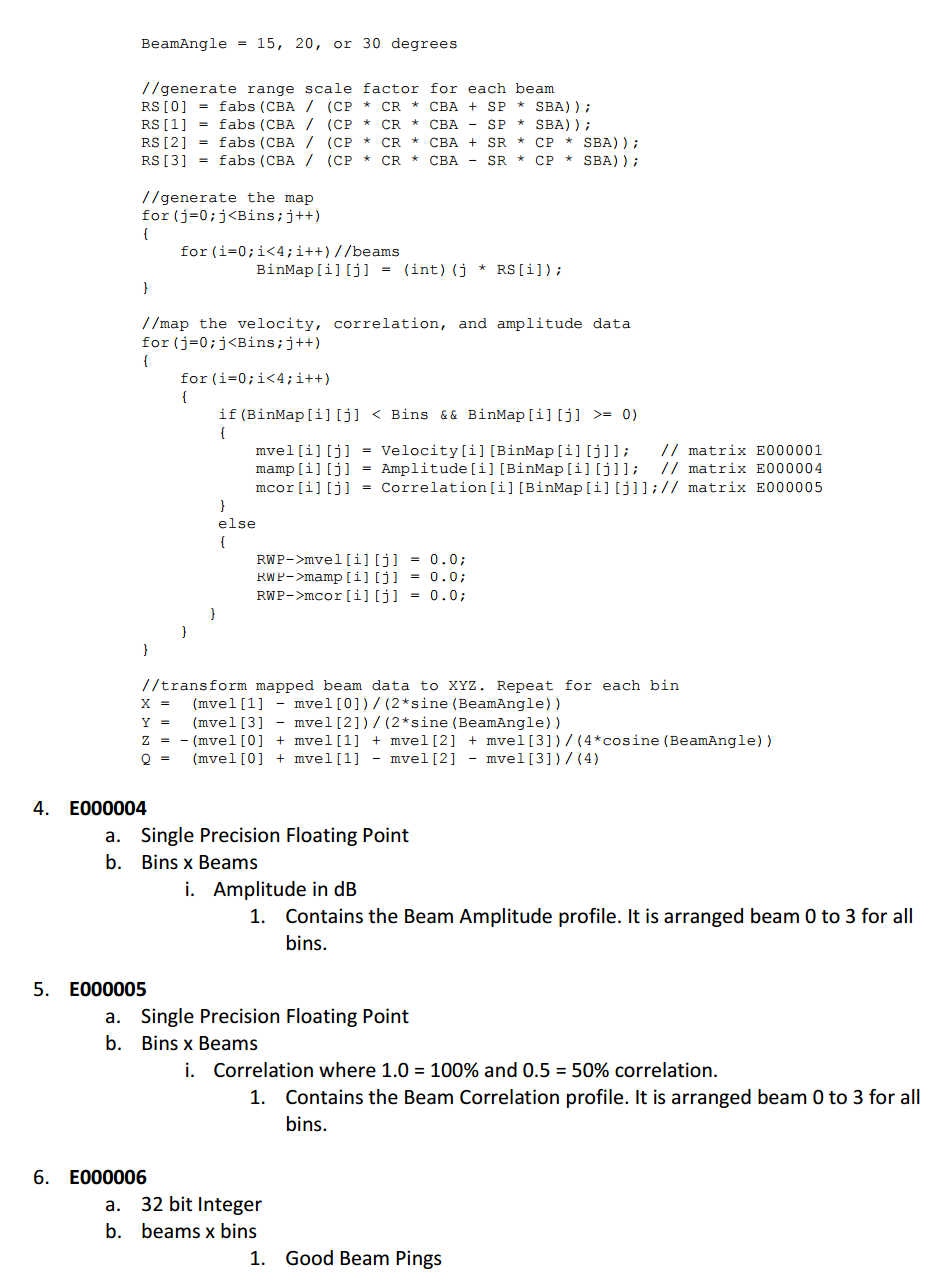
\includegraphics[width=1\textwidth]{ens2}
\end{figure}
\begin{figure}[ht]
\centering
      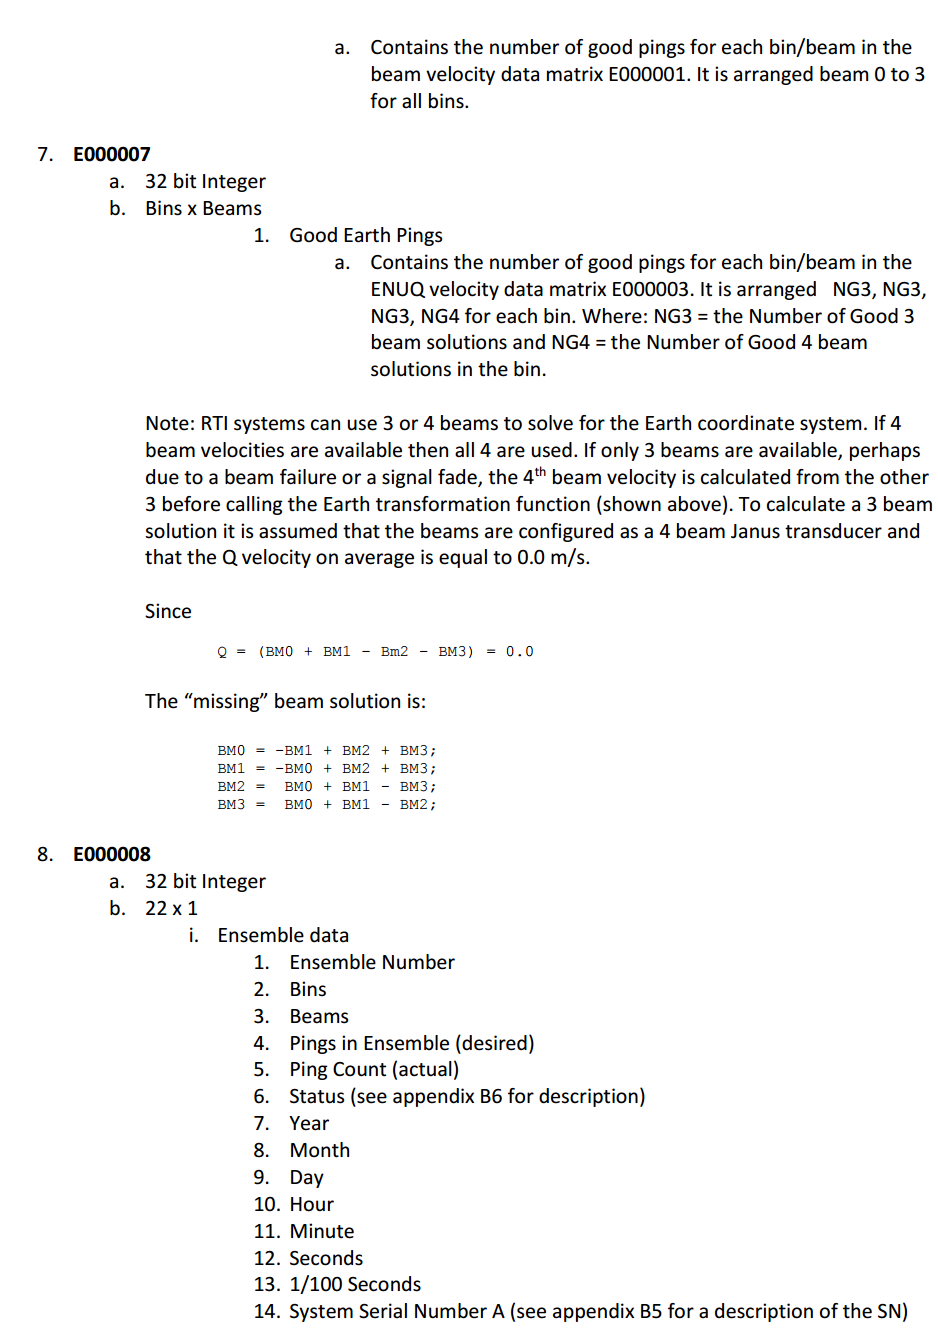
\includegraphics[width=1\textwidth]{ens3}
\end{figure}
\begin{figure}[ht]
\centering
      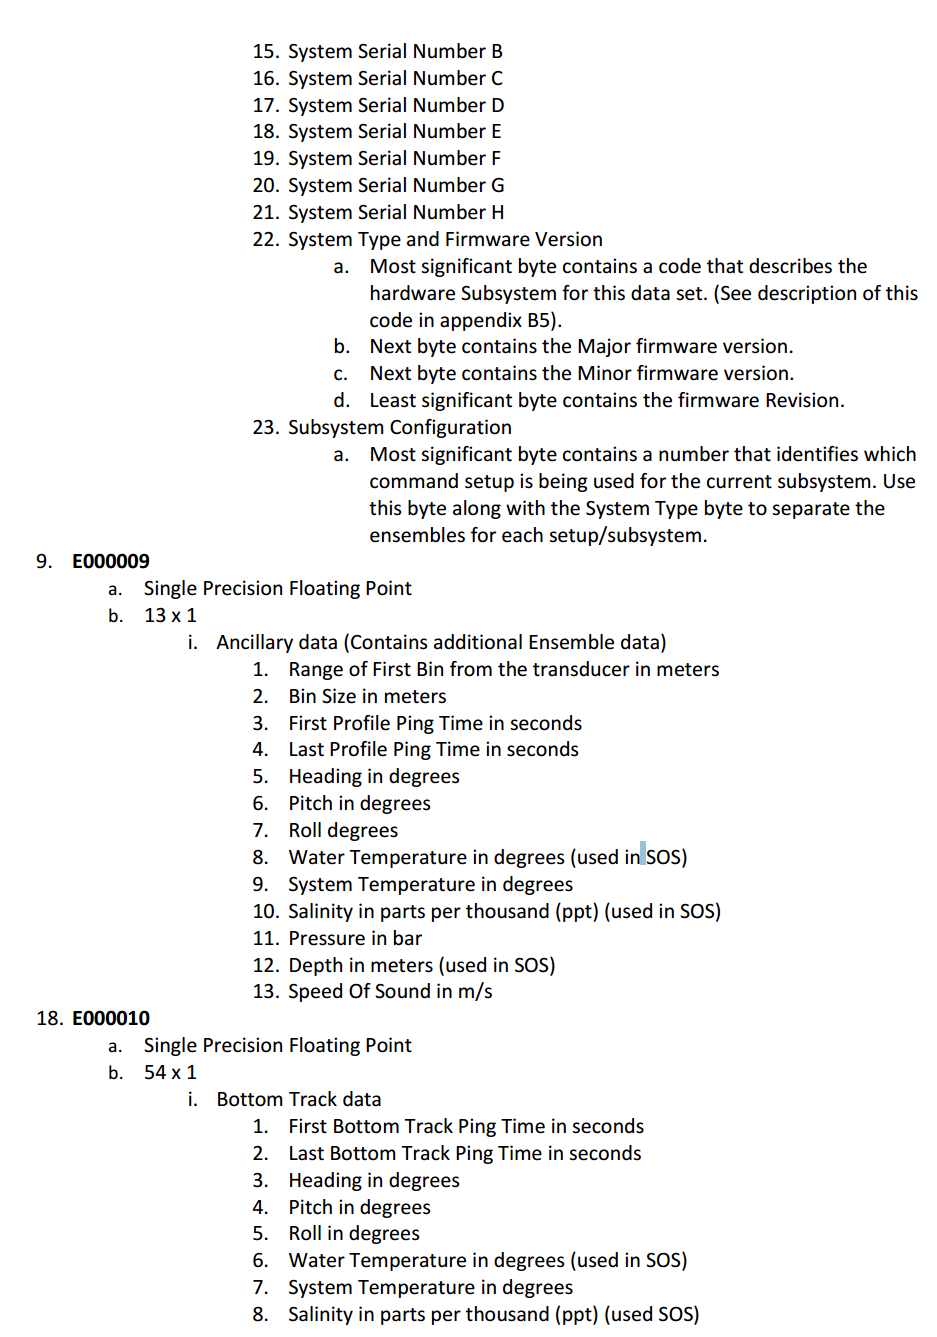
\includegraphics[width=1\textwidth]{ens4}
\end{figure}
\begin{figure}[ht]
\centering
      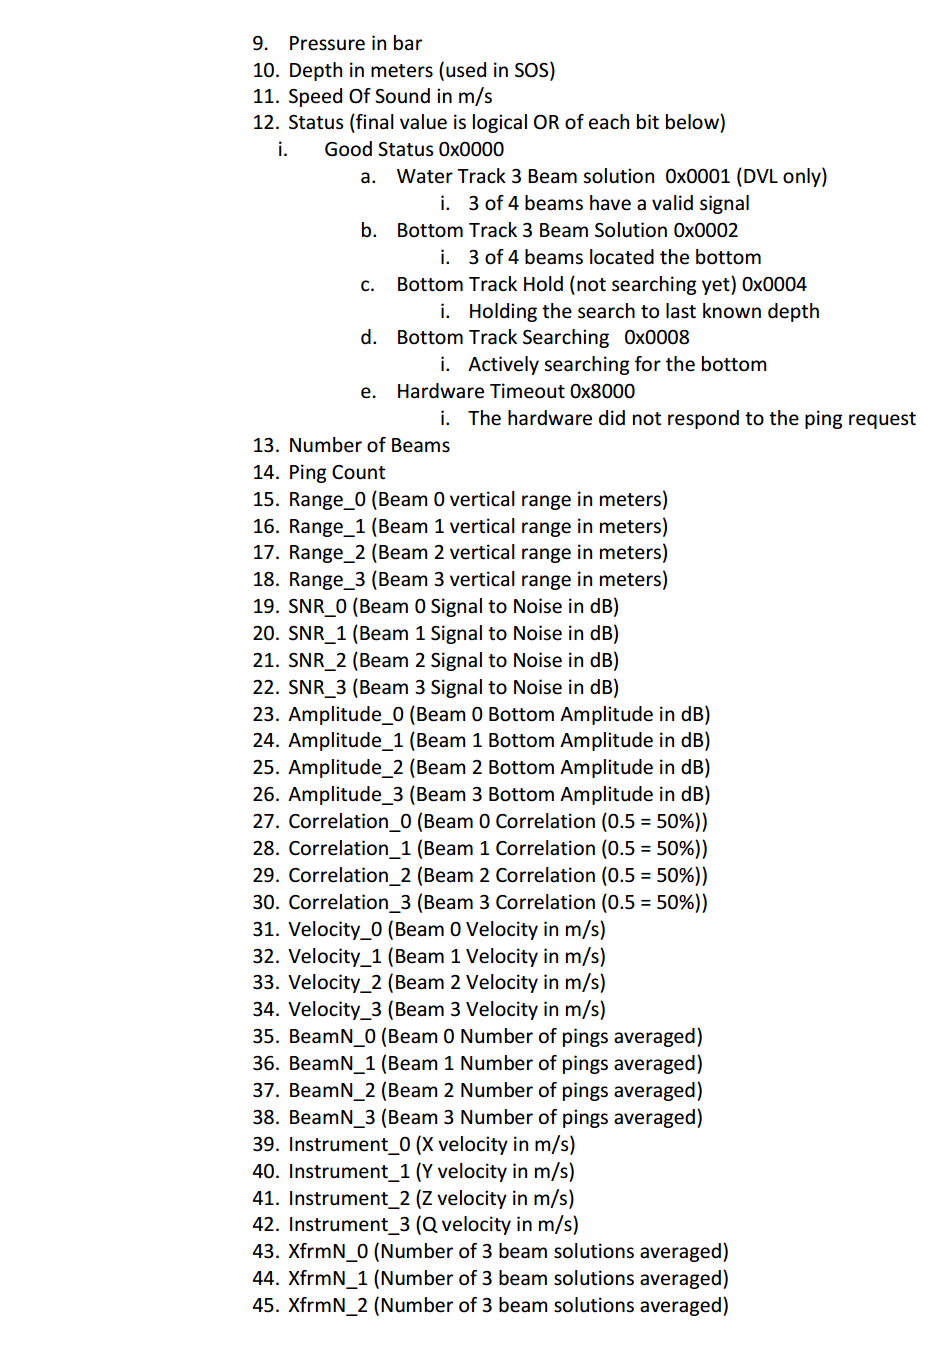
\includegraphics[width=1\textwidth]{ens5}
\end{figure}
\begin{figure}[ht]
\centering
      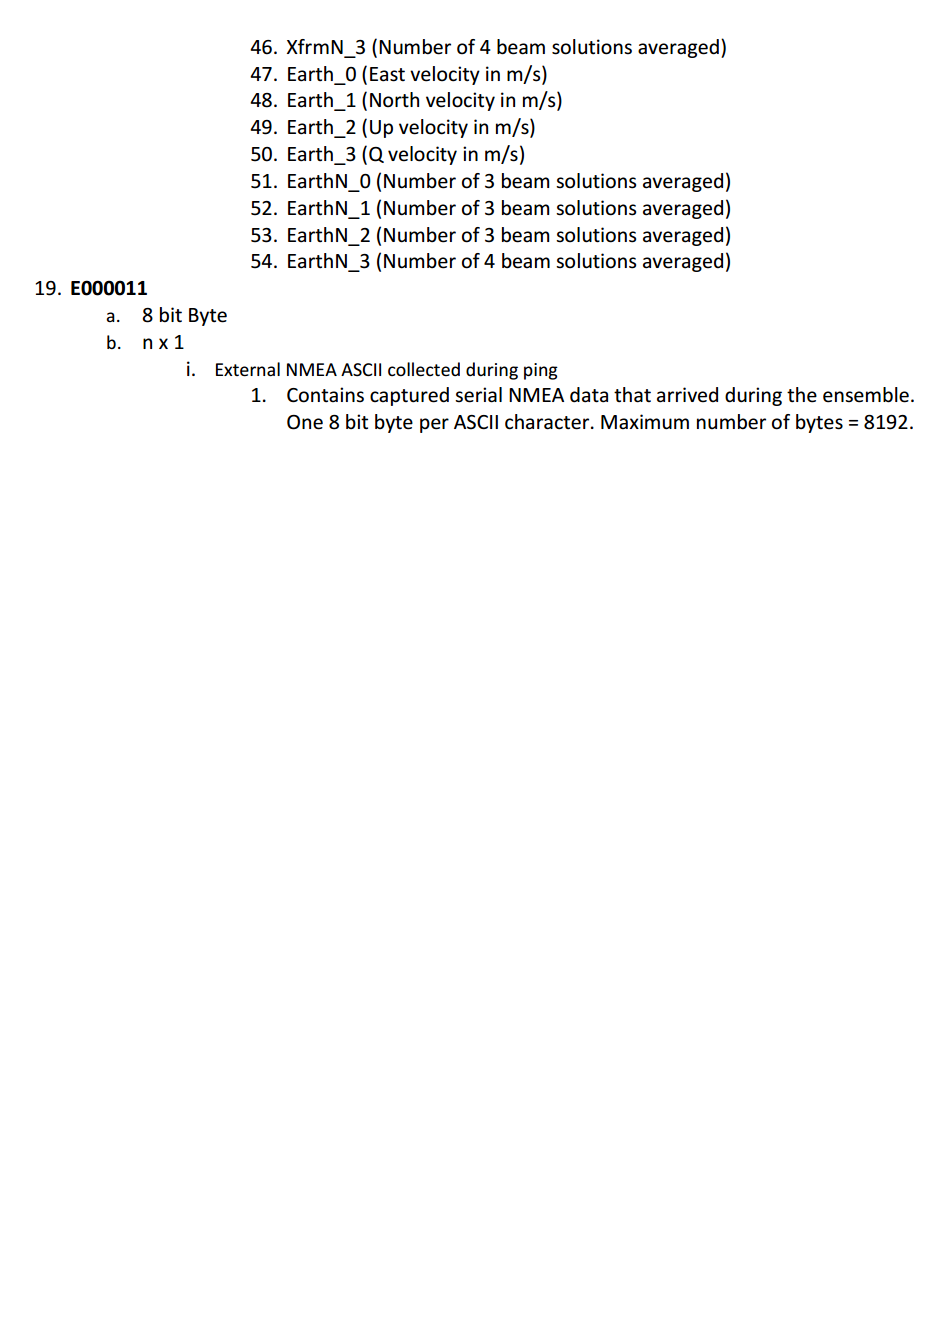
\includegraphics[width=1\textwidth]{ens6}
\end{figure}
\begin{figure}[ht]
\centering
      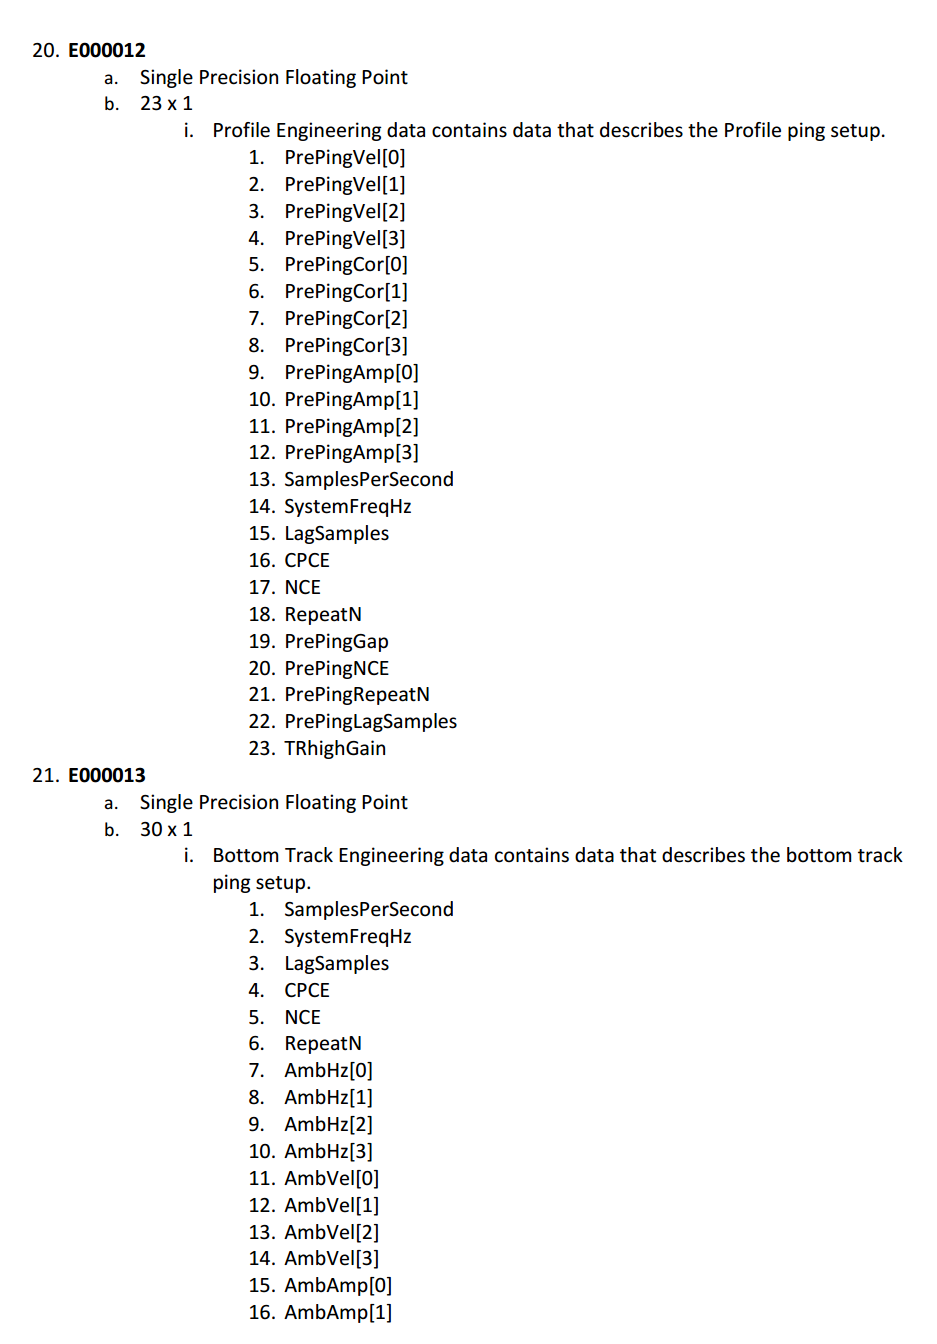
\includegraphics[width=1\textwidth]{ens7}
\end{figure}
\begin{figure}[ht]
\centering
      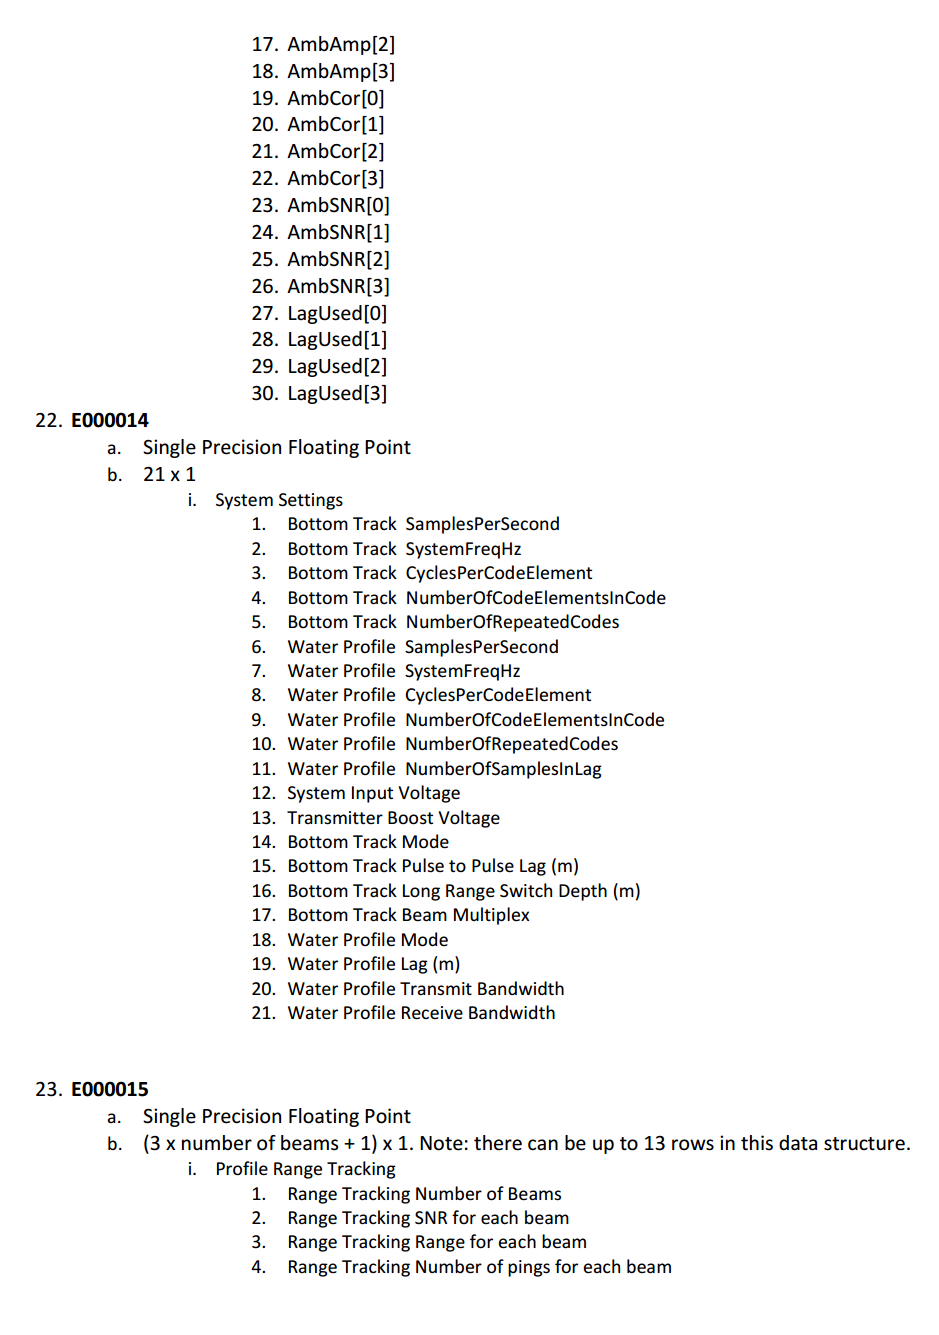
\includegraphics[width=1\textwidth]{ens8}
\end{figure}

\chapter{ADCP Burst Generator}
The source code used to generate ADCP bursts, and send them over a serial port.
\lstset{basicstyle=\tiny}
\begin{lstlisting}[language=C++]
/********************************************************
 * File:   createBurst.h
 * Author: Christian Ott
 * Created on April 15, 2016
 *
 * Copyright (c) 2016, General Acoustics e.K.
 * Redistribution and use in source and binary forms, with or without modification, are permitted!
 *
 * 2016-06-29 v1.00: First Release
 *
 * *****************************************************/

#ifndef ADCP_LOGGER_CREATEBURST_H
#define ADCP_LOGGER_CREATEBURST_H

#include <vector>
#include <chrono>
#include "../src/AdcpDataSet.h"
#include "../src/AdcpLogger.h"
#include "../src/MatlabUtils.h"

using ByteVec = std::vector<unsigned char >;
using TimeStamp = std::chrono::system_clock::time_point;
using Int32Vec = std::vector<int32_t>;
using Float32Vec = std::vector<boost::float32_t>;
using MessageVec = std::vector<BinaryMessage>;
struct ErrorConfig{
    int doubleheader;
    int doublestartseq;
    int startseqshort;
    int halfens;
    int missingbyte;
};

MessageVec createBurst(uint32_t stertEnsNr, TimeStamp ts, uint32_t numOfEns, ErrorConfig err );

ByteVec createSmallFrame(TimeStamp ts, uint32_t ensNr);
ByteVec createBigFrame(TimeStamp ts, uint32_t ensNr);

static Int32Vec generateRandomIntVec(size_t size);
static Float32Vec generateRandomFloatVec(size_t size);

#endif //ADCP_LOGGER_CREATEBURST_H

\end{lstlisting}
\pagebreak

\begin{lstlisting}[language=C++]
/********************************************************
 * File:   createBurst.cpp
 * Author: Christian Ott
 * Created on April 15, 2016
 *
 * Copyright (c) 2016, General Acoustics e.K.
 * Redistribution and use in source and binary forms, with or without modification, are permitted!
 *
 * 2016-06-29 v1.00: First Release
 *
 * *****************************************************/
#include <boost/thread.hpp>
#include "createBurst.h"
#include "../src/AdcpLogger.h"
#include "../external/SerialPort.h"
#include "../src/BinaryIO.h"
void runOutput(std::string com, uint32_t baud, MessageQueue &istream);
void runGenerator(MessageQueue &istream);
ByteVec createSmallFrame(TimeStamp ts, uint32_t ensNr);
ByteVec createBigFrame(TimeStamp ts, uint32_t ensNr);
MessageVec createBurst(uint32_t stertEnsNr, TimeStamp ts, uint32_t numOfEns, uint32_t delta, bool err );

int main(int argc, char* argv[]) {

    moodycamel::ConcurrentQueue<BinaryMessage, moodycamel::ConcurrentQueueDefaultTraits> MessageQueue(200);

    std::string com = argv[1];
    uint32_t baud =  std::stoi(argv[2]);

    boost::thread ensGenerator(runGenerator,std::ref(MessageQueue));
    boost::thread outputThread(runOutput, com, baud, std::ref(MessageQueue));

    ensGenerator.join();
    outputThread.join();
}
void runOutput(std::string com, uint32_t baud, MessageQueue &istream){
    SerialPort serial(com,baud);

    bool exitLoop = false;
    moodycamel::ConsumerToken ct(istream);
    while(!exitLoop){
        BinaryMessage msg;
        if(istream.try_dequeue(ct,msg)) {
            serial.write((const char *) &msg.getDataP()->data()[0], msg.getDataP()->size());
        }
    }
    serial.close();
}

void runGenerator(MessageQueue &istream){
    auto ts = TimeUtils::string_to_time_point("2016-06-15 02:02:00.00");
    auto ensnr = 20;
    while(1){

        auto burst = createBurst(ensnr,ts,2048,200,false);
        for(auto b : burst){
            istream.enqueue(b);
            boost::this_thread::sleep(boost::posix_time::milliseconds(2));
        }
        boost::this_thread::sleep(boost::posix_time::seconds(20));
        ts += std::chrono::minutes(10);
        ensnr +=2048;
    }
}
MessageVec createBurst(uint32_t stertEnsNr, TimeStamp ts, uint32_t numOfEns, uint32_t delta, bool err ){
    auto ensnr = stertEnsNr;
    auto tts = ts;
    std::random_device rd;     // only used once to initialise (seed) engine
    std::mt19937 rng(rd());    // random-number engine used (Mersenne-Twister in this case)
    std::uniform_int_distribution<int> uni(1,numOfEns); // guaranteed unbiased

    auto rand = uni(rng);
    MessageVec vec;

    while( numOfEns > 0){
        ByteVec frame;
        if((numOfEns % 2) == 0){
            frame = createSmallFrame(tts, ensnr);
        } else{
            frame = createBigFrame(tts, ensnr);
        }

        if (numOfEns == rand && err) {
            frame.insert(frame.begin(),frame.begin(),frame.begin()+32);
        }
        BinaryMessage m(tts,std::move(frame));
        vec.push_back(std::move(m));
        ensnr++;
        tts += std::chrono::milliseconds(delta);
        numOfEns--;
    }
    return std::move(vec);
}


ByteVec createSmallFrame(TimeStamp ts, uint32_t ensNr){
    AdcpEnsemble ensemble;
    ensemble.matrices.insert({"E000001", std::make_shared<E01>()});
    std::dynamic_pointer_cast<ExxFloat32>(ensemble.matrices["E000001"])->setVector(
            generateRandomFloatVec(30),
            30,
            1);


    ensemble.matrices.insert({"E000004", std::make_shared<E04>()});
    std::dynamic_pointer_cast<ExxFloat32>(ensemble.matrices["E000004"])->setVector(
            generateRandomFloatVec(30),
            30,
            1);

    ensemble.matrices.insert({"E000005", std::make_shared<E05>()});
    std::dynamic_pointer_cast<ExxFloat32>(ensemble.matrices["E000005"])->setVector(
            generateRandomFloatVec(30),
            30,
            1);

    ensemble.matrices.insert({"E000006", std::make_shared<E06>()});
    std::dynamic_pointer_cast<ExxInt32>(ensemble.matrices["E000006"])->setVector(
            generateRandomIntVec(30),
            30,
            1);

    auto e8vec = generateRandomIntVec(23);
    e8vec[0] = ensNr;
    e8vec[1] = 30;
    e8vec[2] = 1;
    auto ts_time = std::chrono::system_clock::to_time_t(ts);
    auto ts_sec = std::chrono::system_clock::from_time_t(ts_time);
    std::chrono::milliseconds ms = std::chrono::duration_cast<std::chrono::milliseconds>(ts - ts_sec);
    std::tm * ttm = localtime(&ts_time);

    e8vec[6] = ttm->tm_year+1900;
    e8vec[7] = ttm->tm_mon+1;
    e8vec[8] = ttm->tm_mday;

    e8vec[9] = ttm->tm_hour;
    e8vec[10] = ttm->tm_min;
    e8vec[11] = ttm->tm_sec;

    e8vec[12] = ms.count()/10;
    ensemble.matrices.insert({"E000008", std::make_shared<E08>()});
    std::dynamic_pointer_cast<ExxInt32>(ensemble.matrices["E000008"])->setVector(
            std::move(e8vec),
            23,
            1);

    ensemble.matrices.insert({"E000009", std::make_shared<E09>()});
    std::dynamic_pointer_cast<ExxFloat32>(ensemble.matrices["E000009"])->setVector(
            generateRandomFloatVec(13),
            13,
            1);

    ensemble.matrices.insert({"E000014", std::make_shared<E14>()});
    std::dynamic_pointer_cast<ExxFloat32>(ensemble.matrices["E000014"])->setVector(
            generateRandomFloatVec(23),
            23,
            1);

    ensemble.matrices.insert({"E000015", std::make_shared<E15>()});
    std::dynamic_pointer_cast<ExxFloat32>(ensemble.matrices["E000015"])->setVector(
            generateRandomFloatVec(4),
            4,
            1);

    AdcpConverter converter;
    auto frame = converter.ensembleToFrame(&ensemble);
    ByteVec res;
    frame.toByte(&res);
    return std::move(res);
}


ByteVec createBigFrame(TimeStamp ts, uint32_t ensNr){
    AdcpEnsemble ensemble;
    ensemble.matrices.insert({"E000001", std::make_shared<E01>()});
    std::dynamic_pointer_cast<ExxFloat32>(ensemble.matrices["E000001"])->setVector(
            generateRandomFloatVec(30*4),
            30,
            4);

    ensemble.matrices.insert({"E000002", std::make_shared<E02>()});
    std::dynamic_pointer_cast<ExxFloat32>(ensemble.matrices["E000002"])->setVector(
            generateRandomFloatVec(30*4),
            30,
            4);

    ensemble.matrices.insert({"E000003", std::make_shared<E03>()});
    std::dynamic_pointer_cast<ExxFloat32>(ensemble.matrices["E000003"])->setVector(
            generateRandomFloatVec(30*4),
            30,
            4);

    ensemble.matrices.insert({"E000004", std::make_shared<E04>()});
    std::dynamic_pointer_cast<ExxFloat32>(ensemble.matrices["E000004"])->setVector(
            generateRandomFloatVec(30*4),
            30,
            4);

    ensemble.matrices.insert({"E000005", std::make_shared<E05>()});
    std::dynamic_pointer_cast<ExxFloat32>(ensemble.matrices["E000005"])->setVector(
            generateRandomFloatVec(30*4),
            30,
            4);

    ensemble.matrices.insert({"E000006", std::make_shared<E06>()});
    std::dynamic_pointer_cast<ExxInt32>(ensemble.matrices["E000006"])->setVector(
            generateRandomIntVec(30*4),
            30,
            4);

    ensemble.matrices.insert({"E000007", std::make_shared<E07>()});
    std::dynamic_pointer_cast<ExxInt32>(ensemble.matrices["E000007"])->setVector(
            generateRandomIntVec(30*4),
            30,
            4);

    auto e8vec = generateRandomIntVec(23);
    e8vec[0] = ensNr;
    e8vec[1] = 30;
    e8vec[2] = 4;

    auto ts_time = std::chrono::system_clock::to_time_t(ts);
    auto ts_sec = std::chrono::system_clock::from_time_t(ts_time);
    std::chrono::milliseconds ms = std::chrono::duration_cast<std::chrono::milliseconds>(ts - ts_sec);
    std::tm * ttm = localtime(&ts_time);

    e8vec[6] = ttm->tm_year+1900;
    e8vec[7] = ttm->tm_mon+1;
    e8vec[8] = ttm->tm_mday;

    e8vec[9] = ttm->tm_hour;
    e8vec[10] = ttm->tm_min;
    e8vec[11] = ttm->tm_sec;

    e8vec[12] = ms.count()/10;
    ensemble.matrices.insert({"E000008", std::make_shared<E08>()});
    std::dynamic_pointer_cast<ExxInt32>(ensemble.matrices["E000008"])->setVector(
            std::move(e8vec),
            23,
            1);

    ensemble.matrices.insert({"E000009", std::make_shared<E09>()});
    std::dynamic_pointer_cast<ExxFloat32>(ensemble.matrices["E000009"])->setVector(
            generateRandomFloatVec(13),
            13,
            1);

    ensemble.matrices.insert({"E000014", std::make_shared<E14>()});
    std::dynamic_pointer_cast<ExxFloat32>(ensemble.matrices["E000014"])->setVector(
            generateRandomFloatVec(21),
            21,
            1);
    ensemble.matrices.insert({"E000015", std::make_shared<E15>()});
    std::dynamic_pointer_cast<ExxFloat32>(ensemble.matrices["E000015"])->setVector(
            generateRandomFloatVec(13),
            13,
            1);
    AdcpConverter converter;
    auto frame = converter.ensembleToFrame(&ensemble);
    ByteVec res;
    frame.toByte(&res);
    return std::move(res);
}
static Int32Vec generateRandomIntVec(size_t size){
    using value_type = int32_t ;
    // We use static in order to instantiate the random engine
    // and the distribution once only.
    // It may provoke some thread-safety issues.
    static std::uniform_int_distribution<value_type> distribution(
            0,
            10);
    static std::default_random_engine generator;

    std::vector<value_type> data(size);
    std::generate(data.begin(), data.end(), []() { return distribution(generator); });
    return data;
}


static Float32Vec generateRandomFloatVec(size_t size){
    using value_type = boost::float32_t ;
    // We use static in order to instantiate the random engine
    // and the distribution once only.
    // It may provoke some thread-safety issues.
    boost::float32_t min = -1.999f;
    boost::float32_t max = 1.999f;

    static std::uniform_real_distribution<value_type> distribution(
            min,
            max);
    static std::default_random_engine generator;

    std::vector<value_type> data(size);
    std::generate(data.begin(), data.end(), []() { return distribution(generator); });
    return data;
}
\end{lstlisting}
\chapter{Contents of the CD}
\begin{itemize}
\item\textbf{01\_source\_code} - Contains the final source code, as well as a small README in markdown and PDF.
\item\textbf{02\_tex\_report} - Contains the source code of the report, including the images and the final printed PDF.
\item\textbf{03\_presentation} - Contains the pptx from the final presentation.
\item \textbf{04\_other} - Contains various documents and files used for this project.
	\begin{itemize}
		\item \textbf{cd\_label} - The digital DC label used to print the CD's
		\item \textbf{documentation} - The documentation files used for the implementation	
		\item \textbf{measurements} - Measurement results with the according bat scripts
		\item \textbf{raw\_adcp\_data} - A few ADCP files, in case the software needs to be tested.
	\end{itemize}
\end{itemize}


\end{document}
